%! TeX program = lualatex

\documentclass[twoside, 11pt]{extreport}
\usepackage{graphicx}
\usepackage{tikz}

% This package removes paragraph indentation and adds space between paragraphs.
\usepackage{parskip}

\usepackage{silence}
% Silences "LaTeX Font Warning" messages
\WarningFilter{latexfont}{Font shape}
\WarningFilter{latexfont}{Some font shapes}

% This sets the depth of the numbering in the table of contents.
% \setcounter{secnumdepth}{0} % Only chapters numbered
\setcounter{secnumdepth}{1} % Chapters and sections numbered

\usepackage{titlesec}

    \titleformat*{\section}{\large\scshape}
    \titleformat*{\subsection}{\normalsize\itshape}
    
    \interfootnotelinepenalty=10000
    \raggedbottom


\usepackage{tabularray}

\usepackage[hang,flushmargin]{footmisc} 

\usepackage{microtype}

\usepackage{fancyhdr}

% Glossaries config
\usepackage[nopostdot,savenumberlist=true,acronym]{glossaries-accsupp}
\newglossarystyle{mystyle}{%
    \setglossarystyle{list}%
    \renewcommand*{\glossentry}[2]{%
        \small
        \item[\glsentryitem{##1}\glstarget{##1}{\glossentryname{##1}}]%
        \glossentrydesc{##1}\space (##2)%
        % \glsentryuseri{##1} % <- used to insert images
        {
        \ifglshasfield{useri}{##1}{\\ \noindent\makebox[\linewidth][r]{\glsentryuseri{##1}}}{}%
        \ifglshasfield{userii}{##1}{\\ \noindent\makebox[\linewidth][r]{\glsentryuserii{##1}}}{}%
        \ifglshasfield{useriii}{##1}{\\ \noindent\makebox[\linewidth][r]{\glsentryuseriii{##1}}}{}%
        }
        % Short horizontal rule centered between entries
        % \par\noindent\makebox[\linewidth]{\rule{0.25\paperwidth}{0.4pt}}%
    }%
    \renewcommand*{\glsgroupskip}{}%
}
\usepackage{float}
%\usepackage{hyperref}
\usepackage{fancyhdr}
    \setlength{\headheight}{13.6pt}
\usepackage{lilyglyphs}
\usepackage{fontspec}
\usepackage{setspace}
\usepackage{multicol}
\usepackage{xurl}
\usepackage[colorinlistoftodos]{todonotes}
\usepackage[font=small,labelfont=bf]{caption}

%\usepackage[T1]{fontenc}
%\usepackage{tgbonum} %<- nice, 80s looking typeface

%\usepackage[scale=1]{tgadventor} % or helvet
%\usepackage[scale=1]{tgadventor}
%\renewcommand{\familydefault}{\sfdefault}


\usepackage{geometry}
% \geometry{
% letterpaper,
% left=0.8in,
 %right=0.8in,
% top=0.8in,
% bottom=1.25in
% }
\geometry{
  paperheight=8.5in,
  paperwidth=5.5in,
  heightrounded,
  left=0.75in,
  right=0.75in,
  top=0.85in,
  bottom=0.75in
}

% Add space before footnote text
\let\oldfootnote\footnote
\renewcommand\footnote[1]{%
\oldfootnote{\enspace #1}}

% Create new command for ``translation'' footnotes:
\newcommand{\trans}[1]{\circledfootnote{{#1}}}

% ---------- circled footnote setup ----------
\makeatletter
% helper: draw a circle around arbitrary text (works with multi-digit numbers)
\newcommand{\circlednum}[1]{%
  \tikz[baseline=(char.base)] \node[draw, circle, inner sep=0.6pt, line width=0.4pt, font=\tiny] (char) {#1};%
}

% main command: prints a circled superscript at the point of use,
% increments the footnote counter and writes an italicized footnote.
\newcommand{\circledfootnote}[1]{%
  \refstepcounter{footnote}% advance footnote counter (keeps hyperref anchors working)
  \textsuperscript{\circlednum{\thefootnote}}% circled mark in the text
  \begingroup
    % redefine how the footnote text is typeset, so we put our circled mark
    % at the start of the footnote and keep the body in italics.
    \renewcommand{\@makefntext}[1]{%
      \noindent\hangindent=1.8em\hangafter=1\circlednum{\thefootnote}\enspace ##1}%
    \footnotetext{\textit{#1}}% the footnote body (already italicised by the argument)
  \endgroup
}
\makeatother
% ---------- end circled footnote setup ----------

%%%%%%%%%%%%%%%%%%%%%%%% GLOSSARY %%%%%%%%%%%%%%%%%%%%%%%%
% Cleaned glossary entries (all \includegraphics removed)
\makeglossaries

% \newglossaryentry{image}{name={sample image},
%     description={an example image},
%     user1={\protect\BeginAccSupp{Alt=
%     {a boilerplate image used in
%     examples}}\protect\includegraphics
%     [height=20pt]{images/01-gliss.png}\protect\EndAccSupp{}}
% }
\newglossaryentry{pictograms}
{
    name=pictograms,
    description={Representative icons which may be used to designate particular instruments, extended techniques, or other performance parameters.},
    user1={%
        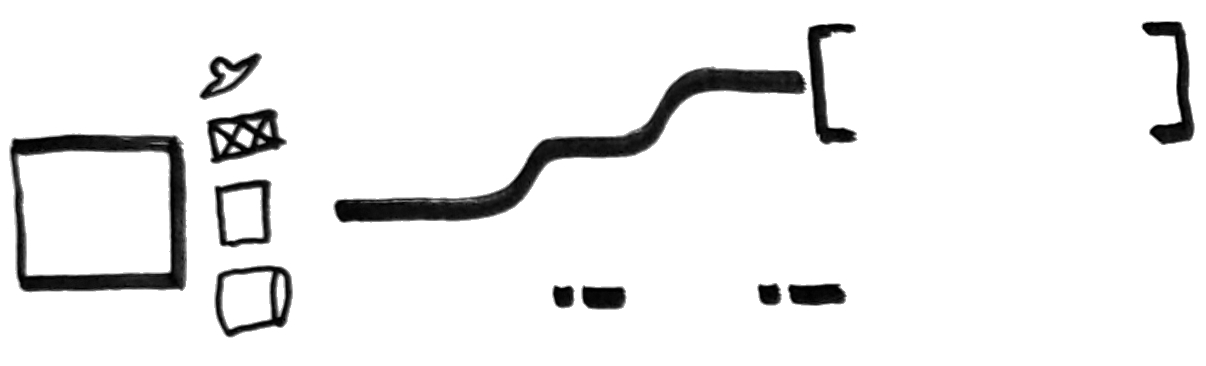
\includegraphics[width=5cm]{images/05-drums2.png}
    },
}
\newglossaryentry{arrow}
{
    name=arrow,
    description={Indicates the continuation of a gesture articulated in the previously enclosed territory. Large decorative arrows indicate transition between one ``sound world'' and another.},
    user1={%
        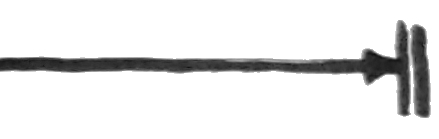
\includegraphics[width=2.5cm]{images/11-arrowplain.png} \hspace*{1cm}
        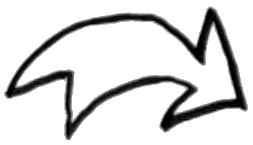
\includegraphics[width=1.5cm]{images/11-elaboratearrow.png}
    },
}

\newglossaryentry{axis}
{ 
    name=axis,
    description={Time is represented on the x-axis; pitch on the y-axis.},
    user1={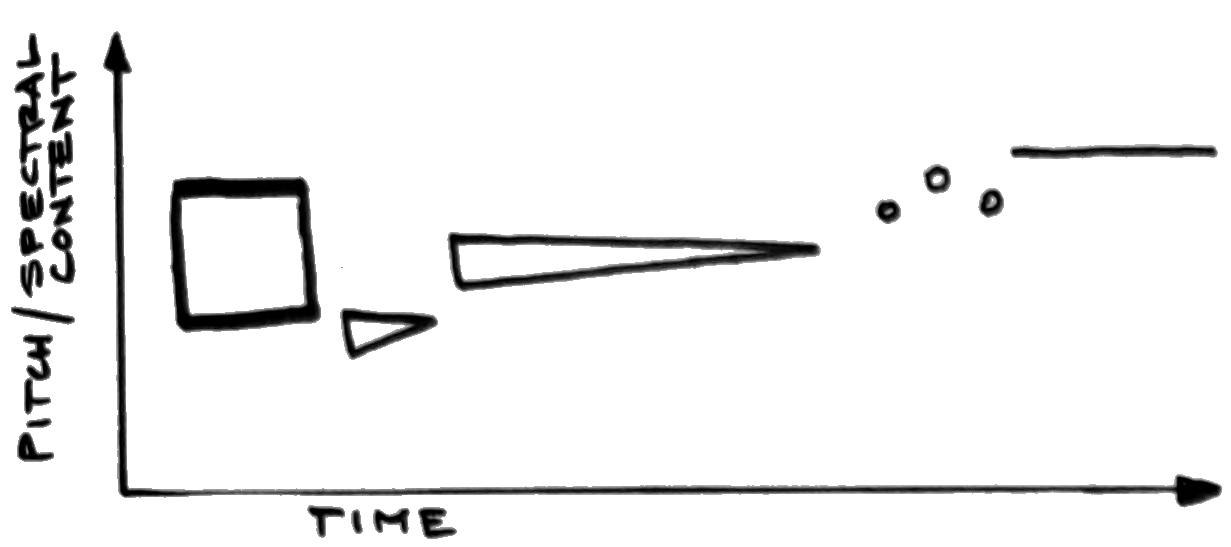
\includegraphics[width=6cm]{images/axesexample.png}},
}

\newglossaryentry{box}
{
    name=box,
    description={Serves as a combined ``clef'' and ``key signature,'' containing information about the following gesture. Top left contains pitch constraints, bottom right contains timbral or gestural constraints.},
    user1={
        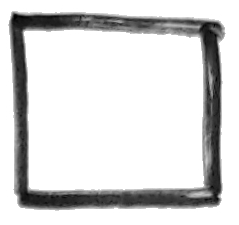
\includegraphics[width=1.5cm]{images/01-box.png} \hspace*{1cm}
        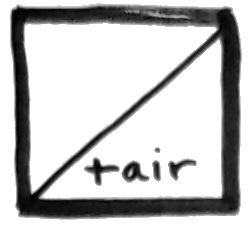
\includegraphics[width=1.5cm]{images/01-boxwithair.png} \hspace*{1cm}
        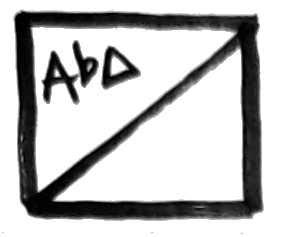
\includegraphics[width=1.5cm]{images/01-boxwithchord.png}
    },
}

\newglossaryentry{brackets}
{
    name=brackets,
    description={Indicate that a gesture is to be played ``in this manner'' rather than note-for-note.},
    user1={%
        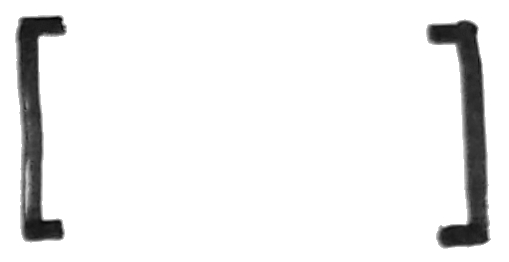
\includegraphics[width=2cm]{images/01-blankbracket.png} \hspace*{1cm}
        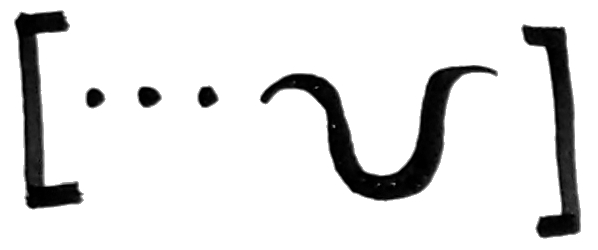
\includegraphics[width=2.5cm]{images/01-3dotscurvebracket.png}
    },
}

\newglossaryentry{line}
{
    name=line,
    description={Indicates an attack of proportional duration. Dashed vertical lines indicate points of simultaneity between two events, two players, etc.},
    user1={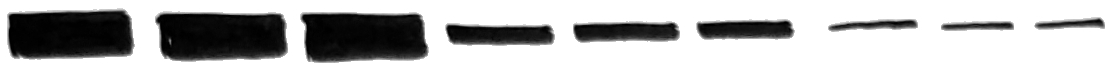
\includegraphics[width=4cm]{images/02-varyingstrokeline.png}}
}


\newglossaryentry{glyphs}
{
    name=glyphs,
    description={Fundamental units of notation; everything besides text is considered a glyph.}
}

\newglossaryentry{dynamics}
{
    name=dynamics,
    description={Indicated using traditional figures (\textit{\textbf{pp}}, \textit{\textbf{mf}}, etc.) or by varying the thickness of the ``stroke'' of the dot, line, or curve. Attack envelopes are demonstrable using changing stroke thickness.},
    user1={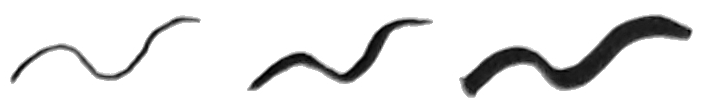
\includegraphics[width=.8\textwidth]{images/02-varyingstrokecurve.png}},
}

\newglossaryentry{timbre}
{
    name=timbre,
    description={Changes in timbre are represented by changes in the visual texture of a dot, line, or curve.},
    user1={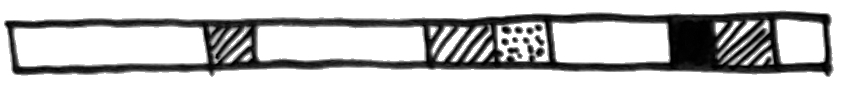
\includegraphics[width=6cm]{images/02-timbre2.png}}
}

\newglossaryentry{lollipop}
{
    name=lollipop,
    description={Used to indicate the relative presence or absence of some parameter specified in the box or elsewhere. Lollipops may be connected by a dashed line indicating a general rate of change.},
    user1={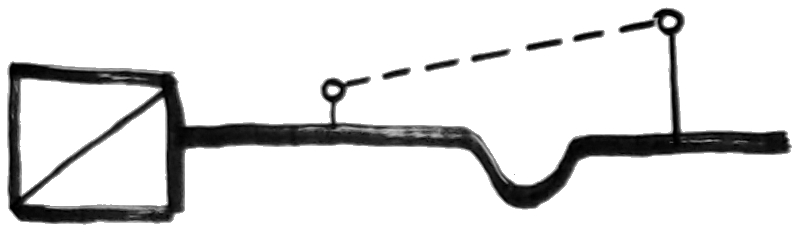
\includegraphics[width=3cm]{images/02-lolly1.png}}
}

\newglossaryentry{relational signs}
{
    name=relational signs,
    description={Come in a wide variety; indicate a specified relationship between two players, two gestures, etc. The referent is indicated with an arrow.},
    user1={%
        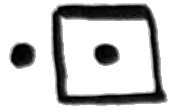
\includegraphics[width=1cm]{images/03-ignore.png} \hspace*{1cm}
        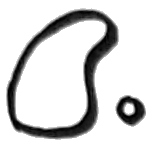
\includegraphics[width=1cm]{images/03-dominate.png} \hspace*{1cm}
        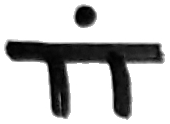
\includegraphics[width=1cm]{images/03-support.png}
    },
}

\newglossaryentry{Pitched material}
{
    name=pitched material,
    description={May be incorporated in a number of ways, ranging from ``fully-notated'' to ``pitches and rhythms'' to ``proportional notation'' to ``pitch classes only.''},
    user1={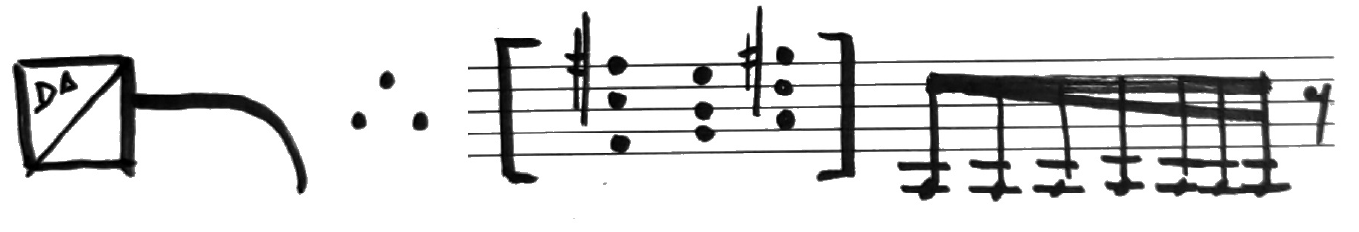
\includegraphics[width=6cm]{images/pitched3.png}}
}

\newglossaryentry{interruption}
{
    name=interruption,
    description={Represented by a center-less asterisk; may be ``in time'' or ``out of time'' (if bracketed).},
    user1={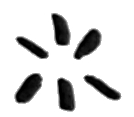
\includegraphics[width=1cm]{images/05-interruption3.png} \hspace*{1cm} 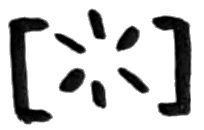
\includegraphics[width=1cm]{images/05-interruption4.png}}
}

\newglossaryentry{multiphonic}
{
    name=multiphonic,
    description={Represented by a pentagonal glyph with or without texture—usually attached to a line indicating duration/dynamic.},
    user1={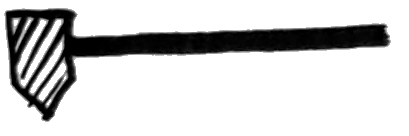
\includegraphics[width=3cm]{images/04-multiphonics3.png}}
}

\newglossaryentry{harmonic}
{
    name=harmonic,
    description={Represented by a small diamond glyph attached to a duration line—understood to be higher than would be indicated by location on the y-axis.},
    user1={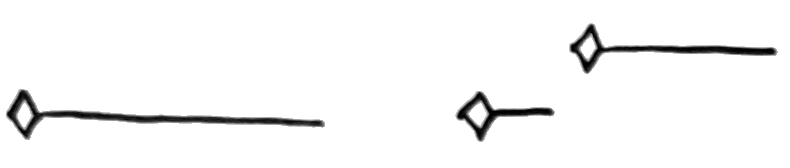
\includegraphics[width=6cm]{images/04-harmonics.png}}
}

\newglossaryentry{chord}
{
    name=chord,
    description={Homophonic material is represented by dots, lines, or curves striated with horizontal bands. Closed/open voicings are indicated by flags attached to the gesture.},
    user1={%
        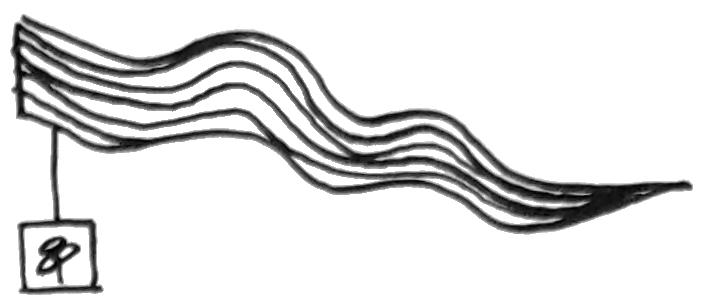
\includegraphics[width=3.5cm]{images/04-chords2.png} \hspace*{1cm}
        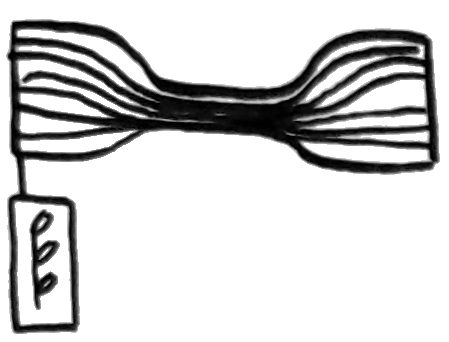
\includegraphics[width=2.5cm]{images/04-chords3.png}
    },
}

\newglossaryentry{duration}
{
    name=duration,
    description={May be indicated either explicitly using timestamps or proportionally using spatial extent.},
    user1={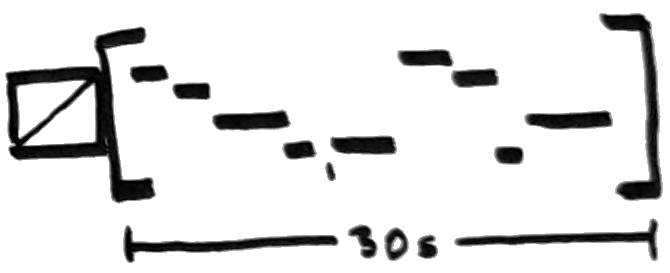
\includegraphics[width=4cm]{images/08-dur2.png}}
}

\newglossaryentry{cue}
{
    name=cue,
    description={Suggested cues are indicated by stars above events or parts of events which are to occur simultaneously.},
    user1={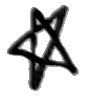
\includegraphics[width=1cm]{images/08-star_alone.png}}
}

\newglossaryentry{trill}
{
    name=trill,
    description={May be notated as a type of curve which oscillates rapidly, or using the traditional \textbf{tr} figure.},
    user1={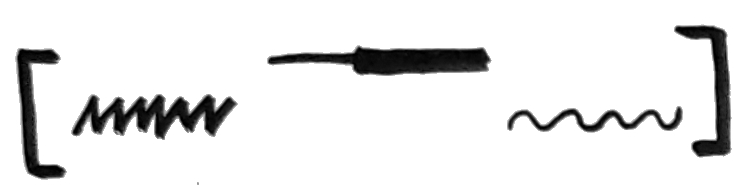
\includegraphics[width=4cm]{images/08-trill2.png}}
}

\newglossaryentry{dot}
{
    name=dot,
    description={A short attack.},
    user1={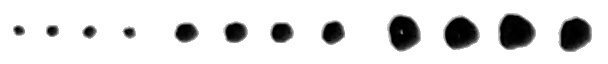
\includegraphics[width=4cm]{images/02-varyingstrokedot.png}}
}

\newglossaryentry{curve}
{
    name=curve,
    description={A series of legato attacks which rises and falls according to the given contour.},
    user1={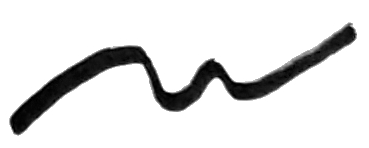
\includegraphics[width=3cm]{images/01-curve2.png}}
}

\newglossaryentry{stroke}
{
    name=stroke,
    description={See \textbf{\gls{dynamics}}.},
}

\newglossaryentry{texture}
{
    name=texture,
    description={See \textbf{\gls{timbre}}.},
}

\newglossaryentry{parameter}
{
    name=parameter,
    description={A musical variable such as pitch, duration, timbre, dynamics, etc.},
}

%\makeglossaries

%\newglossaryentry{axis}
%{
%    name=axis,
%    description=Time is represented on x-axis; pitch on y-axis
%}

%\newglossaryentry{box}
%{
%    name=box,
%    description={$\vcenter{\fbox{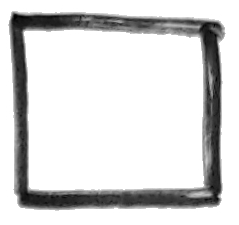
\includegraphics[width=1cm]{images/01-box.png}}}$ \\ serves as a combined ``clef'' and ``key signature,'' containing information about the following gesture}
%    %description={serves as a combined ``clef'' and ``key signature,'' containing information about the following gesture}
%}

%\newglossaryentry{brackets}
%{
%    name=brackets,
%    description={$\vcenter{\protect\fbox{\protect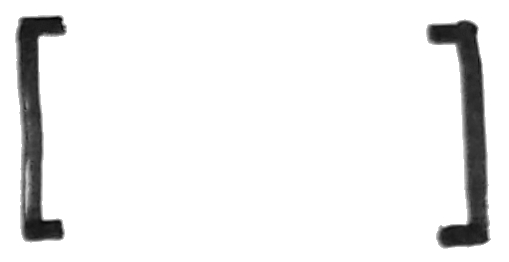
\includegraphics[width=2cm]{images/01-blankbracket.png}}}$ \\ indicate that a gesture is to be played ``in this manner'' rather than note-for-note}
%}

%\newglossaryentry{line}
%{
%    name=line,
%    description={$\vcenter{\protect\fbox{\protect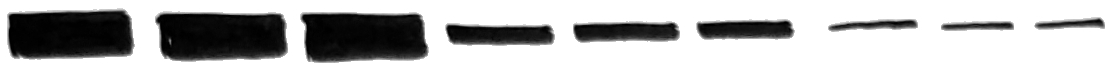
\includegraphics[width=4cm]{images/02-varyingstrokeline.png}}}$ \\ indicates an attack of proportional duration. \textbf{Dashed vertical lines}, on the other hand, indicate points of simultaneity between two events, two players, etc}
%}

%\newglossaryentry{arrow}
%{
%    name=arrow,
%    description={$\vcenter{\protect\fbox{\protect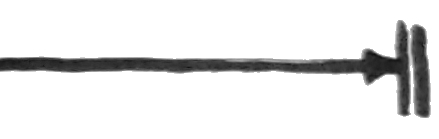
\includegraphics[width=2.5cm]{images/11-arrowplain.png}}}$ \\ indicates the continuation of a gesture as laid out in the previously enclosed territory. \\ \textbf{Large, elaborate arrows} $\vcenter{\fbox{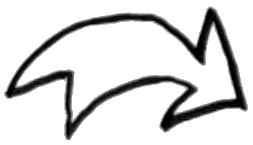
\includegraphics[width=1cm]{images/11-elaboratearrow.png}}}$, on the other hand,  indicate transition between one ``sound world'' and another}
%}

%\newglossaryentry{glyphs}
%{
%    name=glyphs,
%    description={fundamental units of notation; everything besides text is considered a glyph}
%}

%\newglossaryentry{dynamics}
%{
%    name=dynamics,
%    description={$\vcenter{\protect\fbox{\protect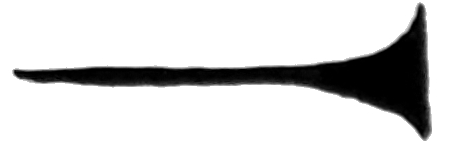
\includegraphics[width=3cm]{images/10-env1.png}}}$ \\ indicated using traditional figures (\textbf{\textit{pp}}, \textbf{\textit{mf}}, etc.) or by varying the thickness of the ``stroke'' of the dot, line, or curve. Attack envelopes are demonstrable using changing stroke thickness}
%}

%\newglossaryentry{timbre}
%{
%    name=timbre,
%    description={$\vcenter{\protect\fbox{\protect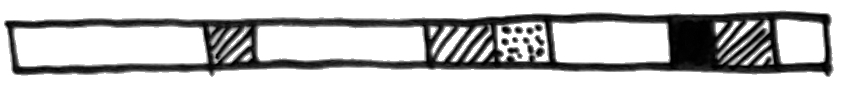
\includegraphics[width=6cm]{images/02-timbre2.png}}}$ \\ changes in timbre are represented by changes in the visual texture of a dot, line, or curve}
%}

%\newglossaryentry{lollipop}
%{
%    name=lollipop,
%    description={$\vcenter{\protect\fbox{\protect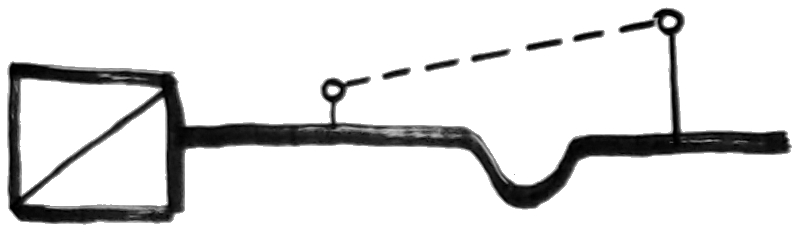
\includegraphics[width=3cm]{images/02-lolly1.png}}}$ \\ used to indicate the relative presence or absence of some parameter specified in the box or elsewhere. Lollipops may be connected by a dashed line indicating a general rate of change}
%}

%\newglossaryentry{relational signs}
%{
%    name=relational signs,
%    description={come in a wide variety; indicate specified relationship between two players, two gestures, etc. Referent will be indicated with an arrow}
%}

%\newglossaryentry{Pitched material}
%{
%    name=pitched material,
%    description={may be incorporated in a number of ways, ranging from ``fully-notated'' to ``pitches and rhythms'' to ``proportional notation'' to ``pitch classes only''}
%}

%\newglossaryentry{interruption}
%{
%    name=interruption,
%    description={$\vcenter{\protect\fbox{\protect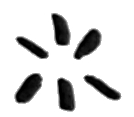
\includegraphics[width=1cm]{images/05-interruption3.png}}}$ \\ represented by a center-less asterisk; may be ``in time'' or ``out of time'' (if bracketed)} 
%}

%\newglossaryentry{multiphonic}
%{
%    name=multiphonic,
%    description={$\vcenter{\protect\fbox{\protect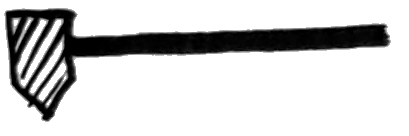
\includegraphics[width=3cm]{images/04-multiphonics3.png}}}$ \\ represented by a pentagonal glyph with or without texture---usually attached to a line indicating duration/dynamic} 
%}

%\newglossaryentry{harmonic}
%{
%    name=harmonic,
%    description={$\vcenter{\protect\fbox{\protect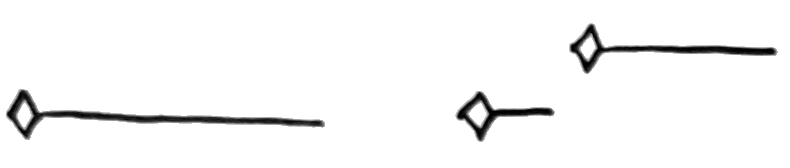
\includegraphics[width=3cm]{images/04-harmonics.png}}}$ \\ represented by a small diamond glyph attached to a line indicating duration/dynamic---understood to be higher than would be indicated by location on y-axis} 
%}

%\newglossaryentry{chord}
%{
%    name=chord,
%    description={$\vcenter{\protect\fbox{\protect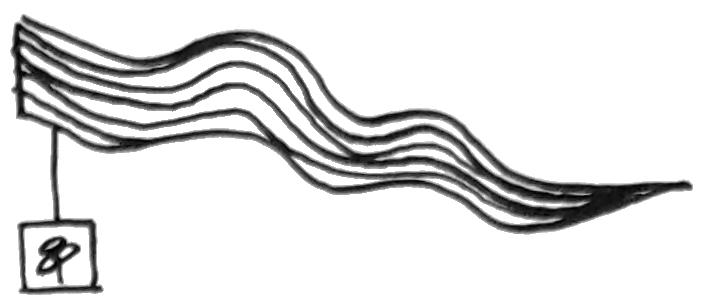
\includegraphics[width=3cm]{images/04-chords2.png}}}$ \\ Homophonic material is represented by dots, lines, or curves striated with horizontal bands. Closed/open voicings indicated by flags attached to gesture} 
%}

%\newglossaryentry{duration}
%{
%    name=duration,
%    description={may be indicated either explicitly using timestamps, etc} 
%}

%\newglossaryentry{cue}
%{
%    name=cue,
%    description={$\vcenter{\protect\fbox{\protect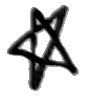
\includegraphics[width=1cm]{images/08-star_alone.png}}}$ \\ Suggested cues are indicated by stars above events or parts of events which are to occur simultaneously} 
%}

%\newglossaryentry{trill}
%{
%    name=trill,
%    description={$\vcenter{\protect\fbox{\protect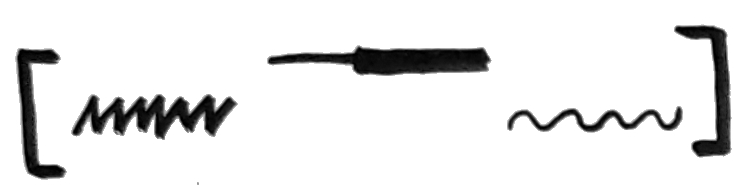
\includegraphics[width=4cm]{images/08-trill2.png}}}$ \\ may be notated as a type of curve which oscillates rapidly or using traditional \textbf{\textit{tr}} figure} 
%}

%\newglossaryentry{dot}
%{
%    name=dot,
%    description={$\vcenter{\protect\fbox{\protect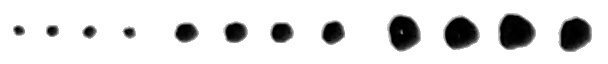
\includegraphics[width=4cm]{images/02-varyingstrokedot.png}}}$ \\ a short attack}
%}

%\newglossaryentry{curve}
%{
%    name=curve,
%    description={$\vcenter{\protect\fbox{\protect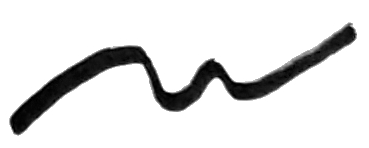
\includegraphics[width=3cm]{images/01-curve2.png}}}$ \\ a series of legato attacks which rises and falls according to the given contour}
%}

%\newglossaryentry{stroke}
%{
%    name=stroke,
%    description={thickness of stroke indicates relative dynamic}
%}

%\newglossaryentry{texture}
%{
%    name=texture,
%    description={the (visual) texture of a dot, line, curve, or other symbol indicates some form of timbral variation, either specified or unspecified}
%}


%%%%%%%%%%%%%%%%%%%%%%%% %%%%%%%% %%%%%%%%%%%%%%%%%%%%%%%%
%\lhead{\includegraphics[width=0.2\textwidth]{nyush-logo.pdf}}


%%%% PROJECT TITLE

\title{\Huge\textbf{ON THE USE AND\\INTERPRETATION OF OTTO-GLYPHS:}\\
        \vspace{.3in}
        \Large \textsc{a brief primer on \\a novel  notation scheme \\for improvising musicians}}

%%%% NAMES OF ALL THE STUDENTS INVOLVED (first-name last-name)
\author{\LARGE{\textsc{isaac otto}}}

\date{\textsc{November 2025 v.1.3}}

\begin{document}
\pagestyle{fancy}
\renewcommand{\chaptermark}[1]{%
\markboth{#1}{}}

\fancyhf{} % clear existing header/footer entries
% We don't need to specify the O coordinate
\fancyhead[OHC]{\textit{Otto-Glyphs}}
\fancyhead[OHR]{\thepage}
\fancyhead[EHC]{\textbf{Ch. \thechapter}}
\fancyhead[EHL]{\thepage}
%\fancyfoot[L]{\thechapter}

\emergencystretch 3em
% (this seems to prevent lines from stretching past margin.)

\maketitle
\tableofcontents
%\thispagestyle{firstpage}
\setstretch{1}
    %\setstretch{1.25} (maybe better?)
\setlength{\marginparwidth}{50pt}


\chapter{Introduction}
\label{ch:intro}

\newpage

Fair warning: this introduction is somewhat wordy and boring. For those who might like to skip straight to the meat of the matter---descriptions of the glyphs themselves begin in \textbf{Chapter \ref{ch:global}}. For the rest of you, please allow the following diversion into the impetus behind this project. 

    \section*{What is this manual for?}

        This small booklet is intended to serve as a general primer introducing performers to a still-developing style of music notation. As much as is possible, I will attempt to spare the reader from paragraphs of ``manifesto''-style pontificating on the whys and wherefores of improvisatory notation and get right to the point: learning to interpret these novel glyphs in the context of a performance. Having said this: if you'll permit me, I'll begin with a brief explanation of the motivation behind the ``system,'' followed by illustrated definitions and contextual examples of the various glyphs which make up its fundamental units. These are organized from most generally-applicable to most specific. Crucially, this is an \textit{ongoing project}. Symbols are apt to change, be added, subtracted, and refined as is deemed necessary for each new piece. This booklet is a snapshot of the state of the project as of Spring 2023 but may (and ought to!) change as rehearsal and performance reveal new desiderata.
    
     %       \begin{itemize}
      %          \item Half manifesto, half primer to get ready to rehearse and perform using this s%         \item After introducing my underlying first principles, we'll first talk through glyphs which you'll find essentially in every context, followed by glyphs which could be considered ``instrument-specific''.
        %        \item Crucially, this is an \textit{ongoing project}. Symbols change and are added, subtracted, and refined as is needed for each new piece. This booklet is a snapshot of the state of the project as of December 2022, but may change (and \textit{should} change) to suit the needs of rehearsal and performance as time goes on.
       %     \end{itemize}

        \section*{Connotative/denotative notation schemes\\\small\textit{how it feels vs. what it says}}

    In the realm of ``graphic'' notation (or, as I prefer, ``neonotation'') there are, broadly considered, two sometimes-intersecting modes of performer engagement: ``connotative'' and ``denotative'' notation schemes. \textbf{Connotative} notation is what I imagine most would think of when the term ``graphic notation'' is mentioned. Perhaps the ur-example of connotative notation is Cornelius Cardew's \textit{Treatise} (1963-67): a sprawling, 193-page score featuring evocatively transfigured staff lines, stems, and beams; stretched nearly beyond recognition into undulating patterned dots, curves, and geometric figures. Famously, Cardew provided no concrete rule-set to facilitate the interpretation of these glyphs. Rather, performers were forced to rely on the connotative content of the symbols themselves to inform their performance tactics---thereby rendering each interpretation a wholly unique ``translation'' of the visual artifact of the score. While Cardew's intent was not necessarily to score \textit{for improvisers}, many 21st-century improv-focused composers take the same tack when crafting their works.

    On the other hand, there exist a small number of more-or-less well-defined \textbf{denotative} notation schemes which imbue their symbols (``graphic'' or otherwise) with enough semantic content that a performer can consistently interpret them from performance to performance. Of these, traditional notation is by far the most prevalent (if trivial) example. However, some recent composers have developed as part of their compositional practice new, robust notational symbologies which have the ability to---for instance---stand in for otherwise unwieldy traditional notation or to constrain the sonic output of improvising musicians (Horatiu Radulescu's ``little devils'' and Anthony Braxton's ``Language Music'' scheme jump to mind). The fledgling system I describe here is decidedly of this latter category. 
    
    Of course, in practice, no system of notation is ever \textit{wholly} connotative or denotative. Since notational symbols are invariably designed to be interpreted by human beings, even the most spartan set of symbols will convey some ``extra-semantic'' meaning over the course of their reading. An angrily-scrawled four-bar passage of quarter-notes has the potential to impart a decidedly different ``flavor'' to the performer (and thereby to the audience) than one that has been delicately engraved on copper plates. As such, a composer who wields a system of graphic notation must always take care to consider potential connotative interpretations of his/her marks on the page.

        
        \section*{What this notation is NOT:}

    This notation is decidedly \textit{not} an attempt to replicate the function of traditional notation. There have been, over the past hundred years or so, several systems which purport to improve upon the venerable five-line staff and its finicky stems, beams, and accidentals. Approaches include giving each chromatic half step $1/12$ of a four-line staff\footnote{See ``Dodeka Notation.''} or switching over to ``stacks'' of six-line octaves\footnote{Various systems shown at \\ \url{https://musicnotation.org/systems/}} in order to do away with flats and sharps entirely. While these may be of some interest to pedagogical min-maxers, traditional notation is, at the end of the day, plenty good enough for its intended purpose.

    Neither, crucially, is this notation a means of ensuring perfect sonic fidelity from performance to performance. While I have no doubt that one could devise a novel, ``semantically weighty'' system of graphic notation which could account for the spectral content of any conceivable sound and thus offer perfect sonic reproducibility, such a Borgesian project would inevitably fail as a notation insofar as the frailty of human perception and recall would stymie its interpretation.
        
    Certainly, the notation I'm proposing here has the ability to, at times, render sonic events in quite fine detail. Ultimately, though, this is a notation oriented toward improvisation first and foremost. As such, there is a built-in promise of some degree of (to use a loaded term) indeterminacy  inherent in any work that employs it---a weakness to be devoutly embraced!

    %        \begin{itemize}
    %          \item Not an attempt to replicate the function of traditional notation!
    %           \item Not a tool for achieving ``accuracy'' or ``sonic fidelity'' between performances!
    %       \end{itemize}
            
        \section*{What this notation IS:}

    Given that we have at our disposal a perfectly serviceable system of extant music notation with which to express our sound- and process-concepts as composers, why burden already-stressed musicians with the responsibility of learning a new set of symbols?
   
    Without doubt, any improvising musician who regularly collaborates with others has experienced a breakdown in communication between some composer (i.e. whoever happens to be tasked with organizing sounds on the bandstand) and the musicians interpreting their desires. The composer may have given only coarse verbal instructions, or they may have drawn a number of evocative, undulating shapes on the page as a source of inspiration---but whatever the case, they feel that their interpreters (being insufficiently clairvoyant) have failed to realize the sound-world they sought to bring about using these methods. At this juncture, barring re-writes, often the only recourse is a sort of fumbling, inadequate descriptive language which may eventually coax a more agreeable performance from the improvisers: ``a little prettier;'' ``pointillist here, then legato;'' ``kinda like that thing you did last week.''

    In short, the symbols I lay out here are one means of more clearly communicating the particulars of where and in what way improvisation ought to take place over the course of a composed work. In addition, they serve, for me, as:
        \begin{itemize}
            \item a means of creatively ``sculpting'' (or ``constraining,'' if you like) the broader space of improvisatory potential;
            \item a means of capturing the gestural essentials of a piece of music, either via transcription or composition;
            \item a means of manipulating \textit{gestural fixity itself} as an independent variable---a way of deliberately scrapping the ``fixed'' music/``open'' music binary.
        \end{itemize}

    These are, of course, weighty claims which ultimately mean very little without clearly delineated examples; many, many of which will come shortly.
    
    %        \begin{itemize}
    %           \item A means of improving communications between composers and improvisers
    %            \item A means of creatively “sculpting” (or “constraining,” if you like) the space of improvisation
    %            \item A means of capturing the gestural essentials of a piece of music (either already-real or as-yet-to-exist)
    %            \item A means of manipulating \textit{gestural fixity itself} as an independent variable — a way of deliberately scrapping the fixed/open binary
    %        \end{itemize}

        \section*{Conducted improvisation v. Otto-Glyphs}

        Many readers will, no doubt, be familiar with at least one of the two popular conducted improvisation methodologies: Butch Morris' ``Conduction'' and Walter Thompson's ``Soundpainting''. To be clear, I will not do these twin systems the justice they deserve by fully explicating their various strengths here. For our purposes, it suffices to say that both systems (which I'll generically lump together as lower-case-c ``conduction'' practices) achieve in real-time many of the tasks I hope to accomplish on the page. To wit: these systems (despite a fascinating measure of ideological opposition between them which I'll explore in some depth in my forthcoming dissertation) both employ a similar demi-hierarchic structure. A ``conductor'' or ``soundpainter'' faces their ensemble and employs a series of predetermined or improvised hand (etc.) gestures which serve as both compulsions to act and as modifiers for said action. One gesture might gently proffer an empty sonic canvas on which a performer might compose---another might radically reduce the improvisatory materials available to a player---a third might force one player's gesture to supervene on another. This polysemic quasi-notation is, in this way, distinct among notations. With a few notable exceptions, notation typically assumes that performance ``begins'' with the null set ($\emptyset$). Traditional notational markings conjure sound from the void; without them, there is only silence. Conduction and Soundpainting certainly have the capacity to function similarly: fine-grained hand gestures exist which may serve to specify particular pitch classes, rhythms, tempi, etcetera. Their radical difference, however, is their ability to bring about the opposite condition (with the wave of a hand, no less!): the composer's medium becomes the set-of-all-sets. That is to say, when the performer is invited to improvise ``freely,'' the composer acts by paring down this now-expanded horizon of sonic potential. We might imagine the difference-in-kind between the sculptor who shapes a clay vessel---\textit{ex nihilo}---by accretion, and the one who---\textit{ex omnis}---pares down a block of alabaster which contains the potential for \textit{all forms}. Conducted improvisation has the unique ability to, in real time, oscillate between and combine these two creative paradigms. In short, this creative synthesis is similiarly the burning core of my project.

        So, again, given that these comparatively successful means of corralling improvisers already exist, why go through the hassle of developing a novel system which, at its heart, strives toward many of the same goals (i.e. the potential for radical co-composition/hierarchic disruption, top down manipulation of improvisatory gesture)? In essence, the trade-off is this: in exchange for the (considerable) richness and flexibility that comes with real-time organization, we gain, in my work, a certain kind of reified musical artifact---one which lends itself far better to archiving; to careful study; to pre-performance inter-musician negotiation. For what it's worth, we gain, too, a visual object; potentially beautiful in its own right. Finally, we gain an organizational structure which facilitates hybridization with the many extant forms of two-dimensional musical notation.
        
        Thus, if the friendly reader is having trouble coming to grips with the general contours of my motivations, it may behoove them to consider this an extension of the intellectual tradition but forward by Morris/Thomson---only committed to paper. In lieu of a real-time participant, the composer (barring his direct musical contribution as an instrumentalist) is relegated to his traditional, silent role; merely setting an elaborate stage for future dialectical collaboration.
        
        \section*{Priorities\\\small\textit{the importance of disobedience}}

    Before delving into the specifics that you, the musician, will encounter on the page, I would like to offer one final qualification which hopefully sheds some light on my priorities:
    
    %While a simple, flexible system such as this one could be deployed in many different ways to suit many different purposes and while, indeed, it is conceivable that one could use the symbols here to merely reproduce the classic hierarchy of composer-over-performer, my goal is precisely the opposite: to build upon the ethos inherent in improvised musics which emphasize co-composition and the \textbf{primacy of the moment}. 
    Any simple, flexible system of notation such as the one I've sought to realize here could certainly be deployed to suit a wide variety of musical/procedural aims. Indeed, it is conceivable that one might, given the right inclination, use this open notation to merely reproduce the traditional composer-over-performer hierarchic paradigm. My goal, however, is precisely the opposite: to build upon the ethos inherent in improvised musics which emphasize co-composition and the \textbf{primacy of the moment}.
    
    That is to say: in performance, musical situations will inevitably arise which seem to demand a gestural contribution that runs counter to what is “prescribed” in the notation. Perhaps the prescribed dynamic is far too timid for the latent energy of the passage; perhaps a sudden rim shot on the floor tom would propel the music into beautiful new territory---a situation unforeseeable prior to performance. As I conceive of it, the primacy of the moment-in-performance \textbf{demands} that the player heed these calls by making a contribution which deliberately ``disobeys'' that which has been laid out by the composer ahead of time. The notation has already “done its job,” so to speak, by sculpting the perceived boundaries of improvisation---it is still incumbent upon \textit{performers} to make the music. I trust the good taste and musical sense of the performer over my prescriptive compositional ability any day. Thus, the performer should allow her in-the-moment judgements to supplement and/or override notational prescriptions should the music demand it. Improvised music is decisively a quasi-democratic pursuit---performers should not be shy about \textit{improvising their musico-social roles} as well as the music itself.

    Now: without any more delay, let's talk about what will show up on the page.

    	
\setcounter{footnote}{0}

        
 
\chapter{Global concepts; all-purpose glyphs}
\label{ch:global}
\newpage

    \section[Axes]{Axes\\\small\textit{the territory upon which we organize gesture}}

            %\begin{figure}[h]
            
            %\vspace{15pt}
            \begin{center}
            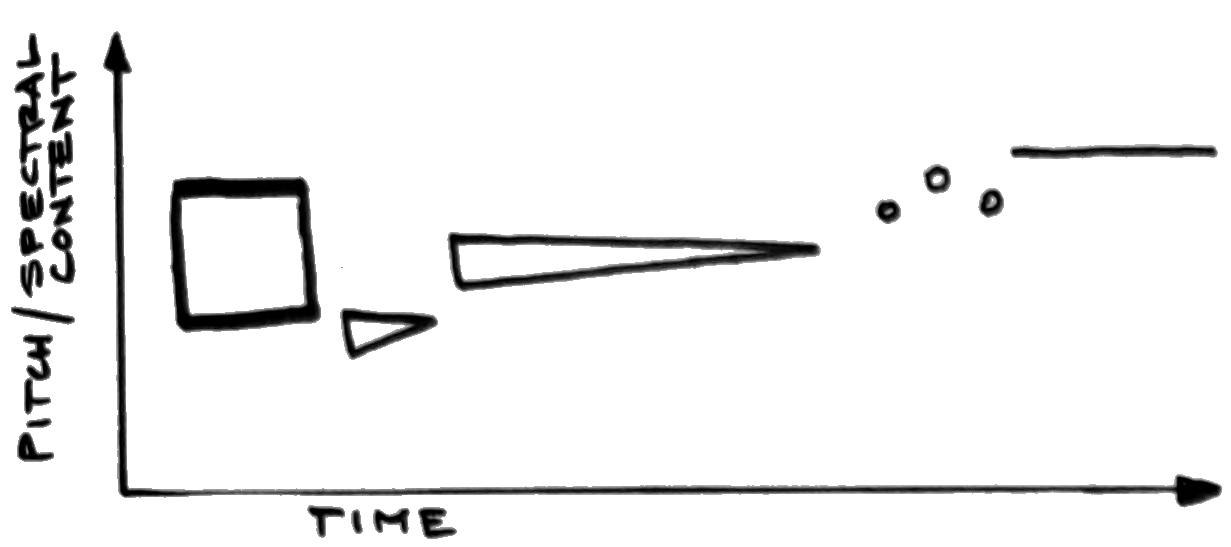
\includegraphics[width=.9\textwidth]{images/axesexample.png}\footnote{When appropriate, I will include italic ``translations'' of the given figures into plain English for reference. In this case, we have \textit{two \textbf{\textit{sfzp}} attacks followed by three \textbf{\textit{p}} staccato attacks and a single \textbf{\textit{pp}} attack}}
            %\caption{A basic illustration of (normally invisible) axes}
            \end{center}
            %\end{figure}

        Groups of \gls{glyphs} are read in what I take to be the most intuitive, natural direction for performers accustomed to traditional notation schemes. Predictably, our x-\gls{axis} is time, which advances from left to right. Time may be encoded in different ways to suit the needs of the piece. In some instances, precise second-to-second changes are specified and are duly marked with time-stamps---necessitating the use of a timekeeping device or more familiarity with the flow of the piece. More often, however, time proceeds ``proportionally,'' whereby the duration of a gesture is only indicated in relation to the overall length of the group of gestures on the page. Performance situations will dictate how long a (for example) two-centimeter-long gesture takes to execute, but as a general rule, a one-centimeter-long gesture should take around half as long. For more information, consult Section 2.2 (\textbf{Duration}).

        The y-axis encodes ``pitch range,'' or, if you like, ``range of spectral content'' which is mapped to the parameters of one's instrument (tempered, of course, by the musician's ability and desires). Generally speaking, glyphs toward the top of the specified territory symbolize higher pitch or spectral content while those toward the bottom symbolize lower frequencies.

        Axes are, of course, not shown on the page but are to be assumed to hold at all times unless otherwise specified.

        \subsection*{A note about pitch height}

        One might reasonably wonder what degree of precision is expected when it comes to interpreting pitch height or (more precisely) pitch \textit{differential} between two glyphs. In short, the system is not set up by default to reproduce precise intervals between attacks. Thus, I find that the best way of interpreting a changing pitch contour is to categorize changes in pitch according to a simple \textbf{``same pitch,'' ``slightly higher/lower,'' ``much higher/lower''} rubric. Again, creativity takes precedence over the rigors of reproduction. Loose observation of contour is sufficient to realize most desired gestures here. If more precision is required,  traditional notation would probably be a better choice.
        
    \newpage
    
    \section[Duration]{Duration\\\small\textit{proportional vs. measured}}

    The duration of a given gesture or individual glyph can be represented in three different ways: \textbf{proportionally}, using \textbf{time stamps} or using \textbf{traditional rhythmic values}. By far the most common method under this scheme is to approach duration \textit{loosely} proportionally. Unlike strict proportional notation where the length of a note (gesture, etc.) on the page has a direct one-to-one correlation with the length of the resulting sound\footnote{See, for instance, Berio's original manuscript for \textit{Sequenza I} for unaccompanied flute}, under this scheme durational stretching and squashing is left up to the performer.

    This is all fine and good for unaccompanied performance, but the problem is complicated by the addition of multiple players who desire some form of synchrony between them. In the context of a duo, trio, etc., proportional durations tend to hold more strictly---though there is, of course, still a good deal of leeway inherent in the system. 
            %\begin{figure}[h]
            \begin{center}
            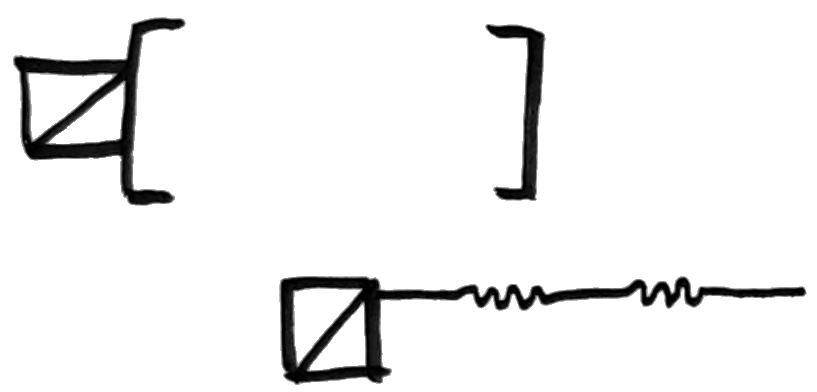
\includegraphics[width=.8\textwidth]{images/08-dur1.png} \circledfootnote{P1 plays open; P2 plays a single pitch which is interrupted by trills}
            %\caption{P2 enters after P1}
            \end{center}
            %\end{figure}

    In the above example, given that there is no additional information present, the precise duration of the bracketed figure is negotiated in real time by Player One (empty bracket) and Player Two (trilling single pitch). Player Two in effect determines the midpoint of the gesture by deciding when to enter. Upon Player Two's entry, Player One then has a strong hint as to when she should conclude her improvisation. This style of notation, of course, works best in small ensembles and when the composer prioritizes performer input and coordination over maximum replicability from performance to performance.

            %\vspace{15pt}
            \begin{center}
            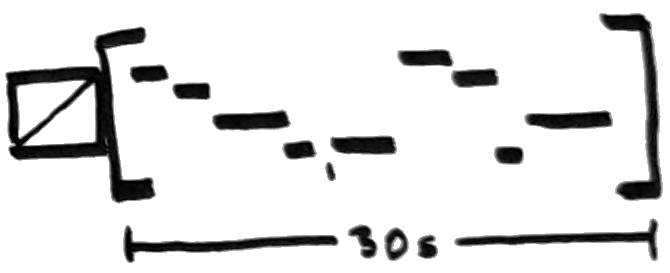
\includegraphics[width=.6\textwidth]{images/08-dur2.png}\circledfootnote{develop something like this arpeggiated gesture for thirty seconds}
            \end{center}

When more precision is desired/required, concrete duration markers may be used to indicate the length of a particular sound/gesture. Depending on how fine-grained these marks are, though, a timekeeping device may become necessary for successful rehearsal or performance---certainly a double-edged sword.

            %\vspace{15pt}
            \begin{center}
            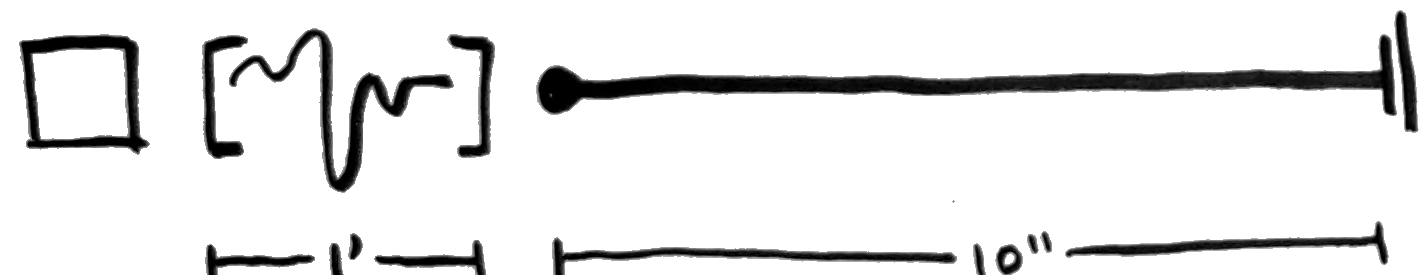
\includegraphics[width=.9\textwidth]{images/08-dur3.png} \circledfootnote{play in-this-manner legato passage for one minute followed by a single tone (\textbf{\textit{sfzp}}) for ten seconds}
            \end{center}

Of course, there is no law stating that the spatial proportions of the glyphs need correspond with the temporal proportions of the sounds they represent. The above graphic illustrates an unexpected arrangement: a small improvised glyph is meant to last for a full minute while the ``longer'' single pitch which follows is a scant 10 seconds\footnote{This is perhaps not ``best practices'' when it comes to engraving technique---but it is decidedly possible. The physical realities of the score-artifact sometimes necessitate creative solutions}. Here, the onus is on the performer to determine the best way to translate the small amount of information given in the first glyph into one minute of sound.

Lastly, duration may be measured according to traditional rhythmic values (\halfNote, \quarterNote, \eighthNote). Glyphs lend themselves to being embedded in traditional notation quite easily---as such, one might find improvisatory gestures occupying staves alongside traditional figures.

            \begin{center}
                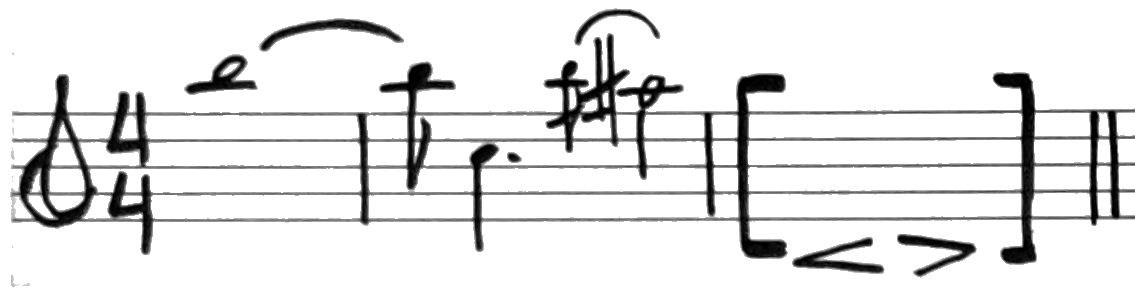
\includegraphics[width=.9\textwidth]{images/09-measure.png}\circledfootnote{play the melodic figure as written, then improvise freely for one measure of~\lilyTimeSignature{4}{4}, first getting louder, then softer.}
            \end{center}

Here, context tells us that the empty set of brackets occupies one full measure of \lilyTimeSignature{4}{4}. Predictably, the composer sacrifices creative leeway here for metric precision. Further, labels may aid in specifying the precise duration of a figure in a rhythmic context, as in the figure below.

            \begin{center}
            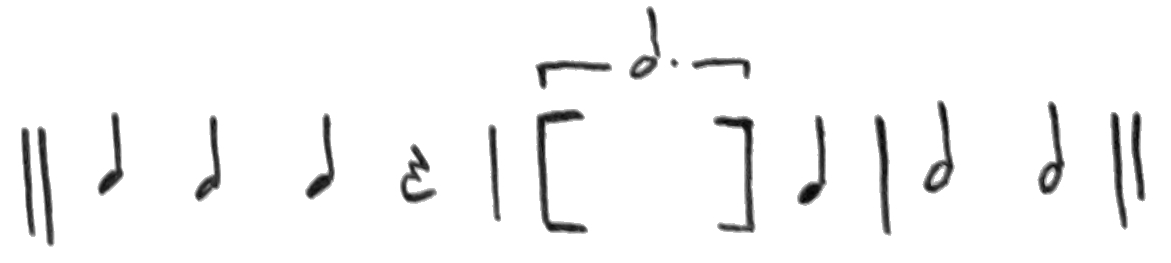
\includegraphics[width=.9\textwidth]{images/09-partialmeasure.png}\circledfootnote{open improvisation for a fixed duration (a dotted half-note) in the context of a metric grid}
            \end{center}






\newpage

    \section[The box]{The box\\\small\textit{gesture-sculpting parameters}}

            \begin{center}
            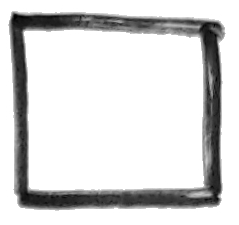
\includegraphics[scale=0.3]{images/01-box.png}\circledfootnote{empty box; no indications}
            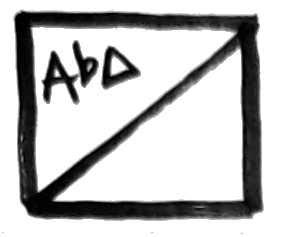
\includegraphics[scale=0.3]{images/01-boxwithchord.png}\circledfootnote{play what follows over [imagined] A$\flat$ major chord}
            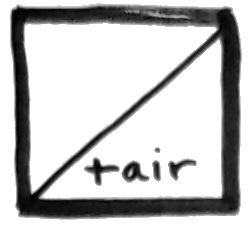
\includegraphics[scale=0.3]{images/01-boxwithair.png}\circledfootnote{the amount of air in your tone will change over the course of this gesture}
            \end{center}
            
        The \textbf{\gls{box}} (sometimes \textbf{box-with-a-slash}) which precedes gestural glyphs serves as a sort of combined ``clef'' and ``key signature'' which may contain modifiers affecting the following gestures. Sometimes its presence merely indicates the beginning of a new group of gestures or a new sound- or process-concept and is thus left empty. 
        
        In the case of the box-with-a-slash, the \textbf{northwest} corner tends to be reserved for parameters which constrain pitch content (e.g. lead sheet symbols like \textbf{E$\flat\Delta{\sharp \textbf{11}}$}, mode indications like \textbf{G Dorian}, or other, more specialized marks\footnote{In the past I have used \textbf{XXIV} to indicate the incorporation of the 24-tone equal-tempered scale---i.e. quarter-tones}. Specific indications here should be spelled out specifically in the performance notes from piece to piece. The \textbf{southeast} corner, on the other hand, is usually used for modifiers which will change in degree or intensity over the course of the gesture group (e.g. amount of air in the sound, amount of ``growl,'' degree of \textit{sul ponticello}, mute position, etc.). For more information see Section 2.9 (\textbf{Lollipops}). 

\newpage

    \section[Bracket notation]{Bracket notation\\\small\textit{a means of modifying gesture's fixity}}

    \begin{center}
    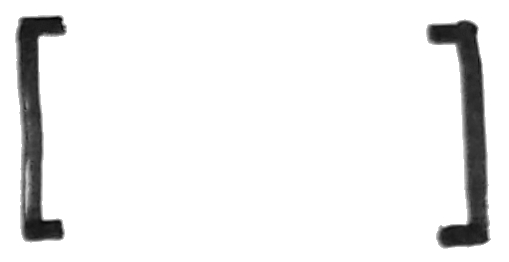
\includegraphics[width=.25\textwidth]{images/01-blankbracket.png}\circledfootnote{{open improvisation}} 
    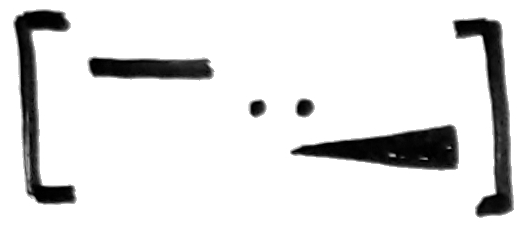
\includegraphics[width=.3\textwidth]{images/01-demobracket.png}\circledfootnote{{play something like this combination of attacks}} 
    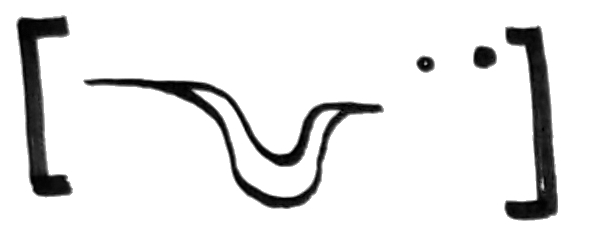
\includegraphics[width=.4\textwidth]{images/01-demobracket2.png}\circledfootnote{{play something like this combination of attacks}}
    \end{center}

        Simple \textbf{\gls{brackets}} are one of our most valuable tools for sculpting an improvised performance. The difference between an un-bracketed and a bracketed gesture is subtle, but makes all the difference in the world. In essence: any time brackets appear, they should be read as: \textbf{play something \textit{in this manner}}. How precisely \textbf{\textit{in this manner}} is interpreted will of course differ greatly between performers. For instance: Where this figure...

            \begin{center}
            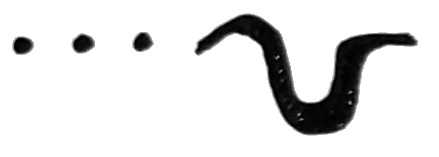
\includegraphics[width=.35\textwidth]{images/01-3dotscurve.png} 
            \end{center}
        
        \noindent indicates \textit{three short attacks and a brief legato passage} across a particular duration, its bracketed counterpart

            \begin{center}
            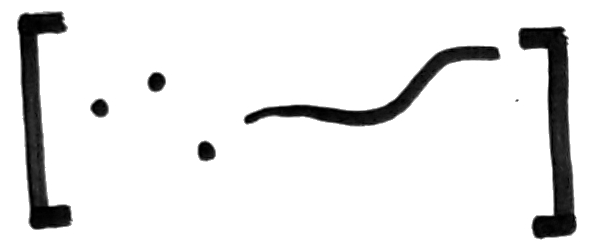
\includegraphics[width=.35\textwidth]{images/01-3dotscurvebracket2.png} 
            \end{center}
        
        \noindent asks the performer to play using these \textit{sorts of} gestures for the duration indicated by the brackets/arrows. Rather than specify certain sounds in certain orders, the bracketed gesture gives a player a sort of ``sonic territory'' to occupy for a given time. The player ought to feel more ``freedom'' with respect to the execution of the material therein than with the more cut-and-dry plain gestures.

        Occasionally a player might run across \textbf{empty brackets}. These serve to indicate that improvisation is essentially unrestricted (except with respect to total duration). Exceptions occur when the empty brackets span only part of the vertical axis... 

            \begin{center}
            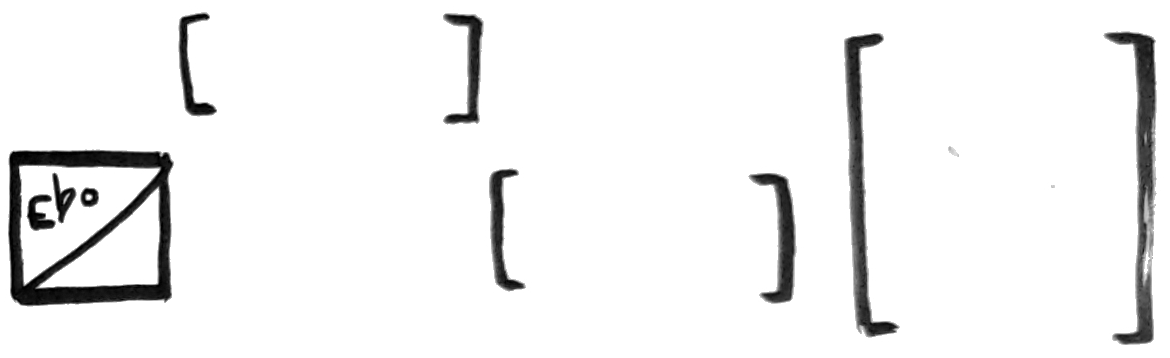
\includegraphics[width=.8\textwidth]{images/05-territory.png}\circledfootnote{{open improvisation across different registers of the instrument, but all over an [imagined] E $\flat$ diminished chord}}
            \end{center}
        
        \noindent which suggest open improvisation emphasizing one portion of the instrument's register. 

        Often, bracketed sections will be extended across the time-axis using a thin, dark \gls{arrow}---especially when only minimal information need be provided in the brackets themselves. This arrow indicates that play continues for the duration. No particular ``development'' of performed material need occur over the duration, though neither is it expressly forbidden.

            \begin{center}
            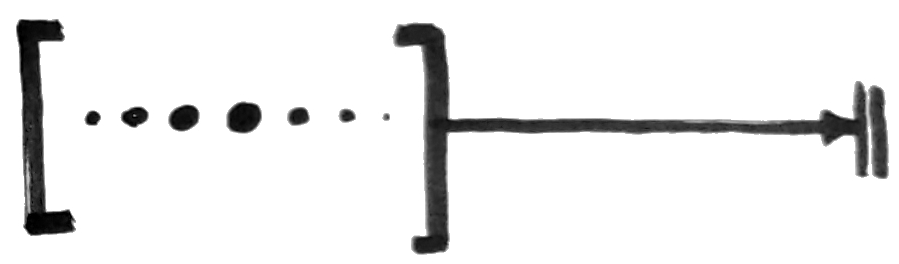
\includegraphics[width=.5\textwidth]{images/01-extarrow.png}\circledfootnote{{repeat something like this \textbf{\textit{pp}} to \textbf{\textit{mp}} gesture until double bar line}}
            \end{center}

\newpage

        

    \section[Dots, lines, and curves]{Dots, lines, and curves\\\small\textit{the fundamental quanta of gesture}}

    %\vspace{15pt}
    
            \begin{center}
            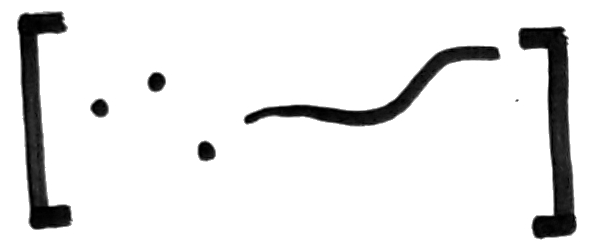
\includegraphics[width=.3\textwidth]{images/01-3dotscurvebracket2.png} \hspace{25pt} 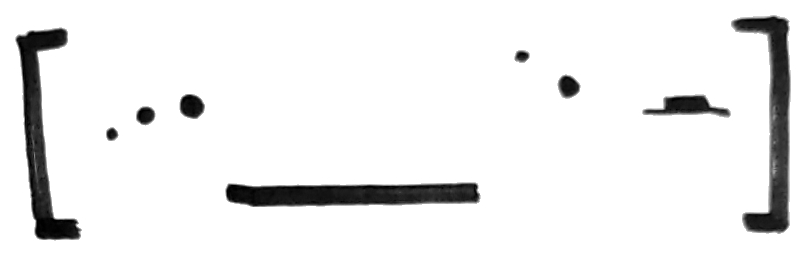
\includegraphics[width=.3\textwidth]{images/01-demobracket3.png} 
            \end{center}
            
            
        The most basic notational sub-units in this scheme are \textbf{\gls{dot}s, \gls{line}s, and \gls{curve}s}. Dots (being in essence very short lines) indicate single short attacks at a particular time (or with a particular density...) Precise attack envelopes (staccato, staccatissimo, tenuto, etc.) are, unless otherwise specified, left to the player's discretion as best befits the performance.

        Straight horizontal lines indicate longer attacks. In the case of percussive or non-sustaining instruments, these might be interpreted as a single attack which decays for the duration or as a stream of attacks in that given pitch-space. 

        I will take care to describe curves in more detail as I take it that despite the intuitiveness of a simple melodic contour, they are apt to be misunderstood. A curve across a given territory has a start, middle, and end point 

            \begin{center}
            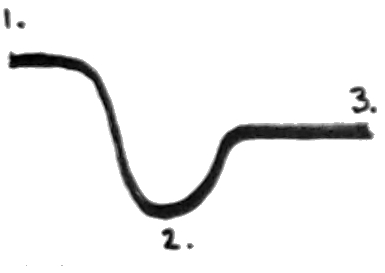
\includegraphics[width=.4\textwidth]{images/01-basiccurve.png}\circledfootnote{{begin high, descend rapidly, end in middle register}}
            \end{center}


            
        \noindent and might be simple or more complex.
        
            \begin{center}
            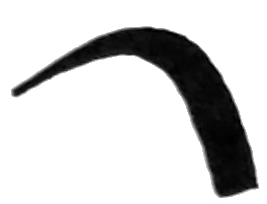
\includegraphics[width=.2\textwidth]{images/01-simplecurve.png}\circledfootnote{{begin quiet, ascend, then rapidly descend while getting louder}} \hspace{25pt} 
            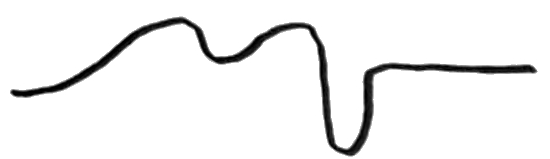
\includegraphics[width=.4\textwidth]{images/01-complexcurve.png}\circledfootnote{{follow this approximate contour}}
            \end{center}
            
            \noindent A curve not otherwise marked could be performed either as a legato stream of notes \textbf{or} as a ``true glissando'' following \textit{roughly} the contour indicated. 
            
            %\vspace{15pt}
            \begin{center}
            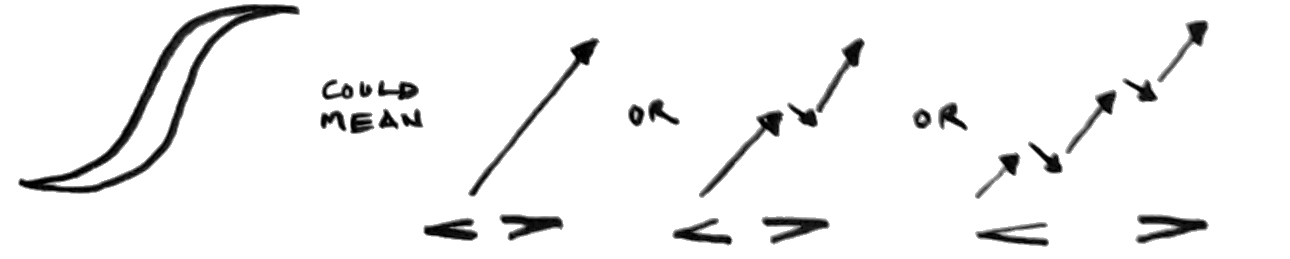
\includegraphics[width=.9\textwidth]{images/01-curvebreakdown.png}
            \end{center}

        It is \textit{not} my intention that the precise ``topography'' of the curve's contour distract the performer from making good music. In all likelihood, the needs of the musical situation might dictate a somewhat different contour than is indicated. The most salient parts of curve gestures are thus their \textbf{duration}, \textbf{start and end points}, and \textbf{relative complexity}.

\newpage

        \subsection{Trills}

        Trills are considered a proper subset of \gls{curve}s---namely curves which demonstrate rapid regular or irregular oscillation with a comparatively short ``wavelength.'' As such, there is no categorical distinction between a ``\gls{trill}'' and a complex curve. Unless otherwise noted, ``trill'' figures are not limited to half- or whole-step oscillation. The figure below demonstrates \textit{a rapid, louder trill, a crescendo on a single tone, then a slower, smoother trill}.

            %\vspace{15pt}
            \begin{center}
            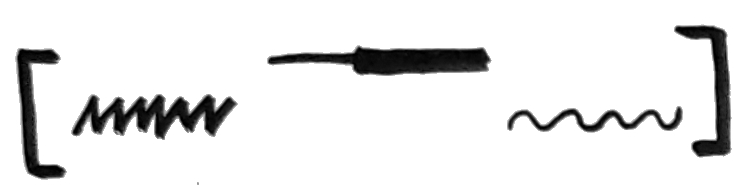
\includegraphics[width=.6\textwidth]{images/08-trill2.png}
            \end{center}        

        Alternately, more conventional trills may be notated using the standard \textbf{\textit{tr}} figure, which may or may not be be accompanied by an interval/direction.

            %\vspace{15pt}
            \begin{center}
            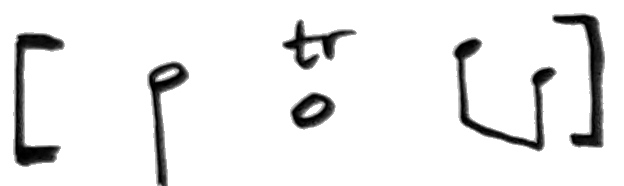
\includegraphics[width=.5\textwidth]{images/08-trill1.png}\circledfootnote{{play something like these rhythms; trill over the longest tone}}
            \end{center}

        

\newpage

        \section[Dynamic indications]{Dynamic indications\\\small\textit{stroke thickness}}
        %\vspace{15pt}

            \begin{center}
            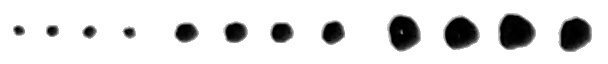
\includegraphics[width=.6\textwidth]{images/02-varyingstrokedot.png} 
            \end{center}

            \begin{center}
            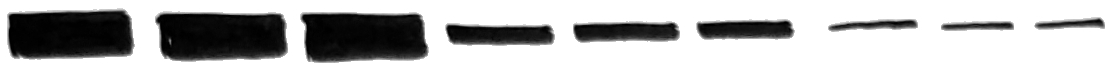
\includegraphics[width=.8\textwidth]{images/02-varyingstrokeline.png} 
            \end{center}

            \begin{center}
            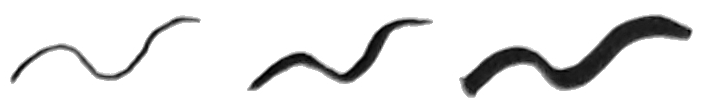
\includegraphics[width=.6\textwidth]{images/02-varyingstrokecurve.png} 
            \end{center}

        Dynamics are communicated in two ways. Traditional \textbf{\textit{pp}} \textbf{\textit{ff}} \textbf{\textit{sffz}}-style \gls{dynamics} as well as \textbf{\textit{\textbf{\textit{cresc}}}} and \textbf{\textit{dim.}} hairpins should be observed as usual. Often, though, when gestural dynamics should vary on a ``note-by-note'' basis, the \textbf{\gls{stroke}}, i.e., the thickness of the \gls{dot}, \gls{line}, or \gls{curve}, will be used to denote dynamic changes. 

        During instances where little to no dynamic information is given (extended sections of uniformly thin lines, for example), the player is encouraged to tweak local dynamics themselves to suit the playing environment. For instance, the figure below need not be performed \textbf{\textit{ppp}} unless directions make it clear.\footnote{This is primarily a caveat included to prevent the engraving of large scores from becoming excessively onerous. Uniformly thin lines are simply easier to render and therefore may stand in for a ``choose-your-own-dynamic'' indication in the absence of other instructions}


            %\vspace{15pt}

            \begin{center}
                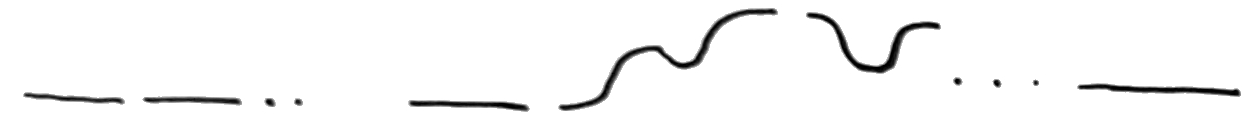
\includegraphics[width=.9\textwidth, angle=1.75]{images/02-thinline.png}\circledfootnote{long and short attacks on one pitch; two longer legato lines followed by several more attacks on a higher pitch}
            \end{center}
            
\newpage
\subsection{Attack envelopes}

    Variations in \gls{stroke} width are often used to indicate specific \textbf{attack envelopes}. These can of course be combined with \textbf{curves}. Below, in no particular order, are a sampling of various possible attack envelopes. The first eight are seen on a single pitch; the final two combine changing attack envelopes with curves/trills.

        \begin{center}
        \begingroup
            \renewcommand{\arraystretch}{4} % Default value: 1
            \begin{tabular}{cc}
            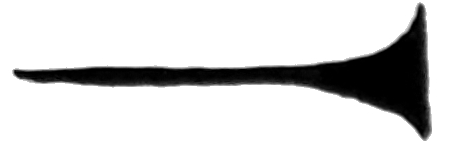
\includegraphics[width=.25\textwidth]{images/10-env1.png} & 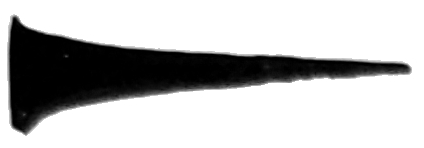
\includegraphics[width=.25\textwidth]{images/10-env2.png} \\
            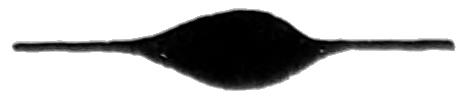
\includegraphics[width=.25\textwidth]{images/10-env3.png} & 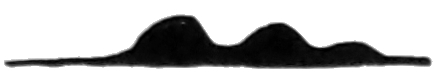
\includegraphics[width=.25\textwidth]{images/10-env4.png} \\
            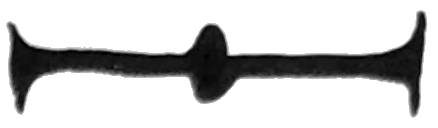
\includegraphics[width=.25\textwidth]{images/10-env5.png} & 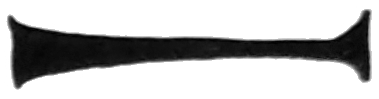
\includegraphics[width=.25\textwidth]{images/10-env6.png} \\
            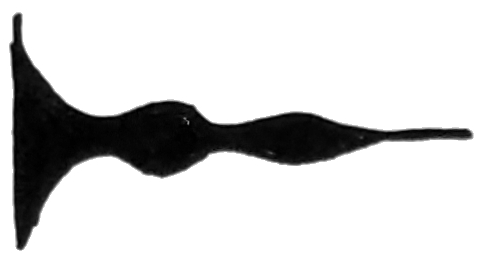
\includegraphics[width=.25\textwidth]{images/10-env10.png} & 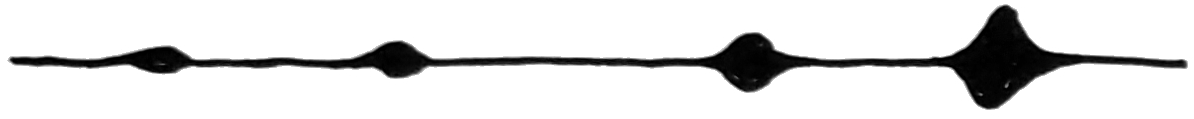
\includegraphics[width=.4\textwidth]{images/10-env7.png} \\
            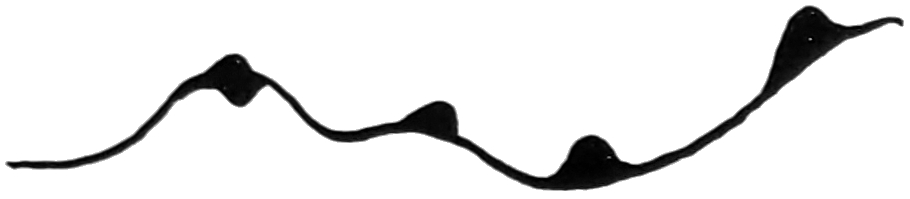
\includegraphics[width=.4\textwidth]{images/10-env8.png} & 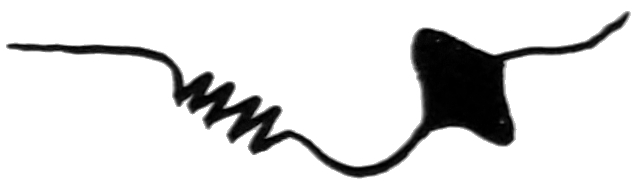
\includegraphics[width=.4\textwidth]{images/10-env9.png} 
            \end{tabular}
        \endgroup
        \end{center}

    %\vspace{15pt}
    
    % \begin{multicols}{2}

            
    %         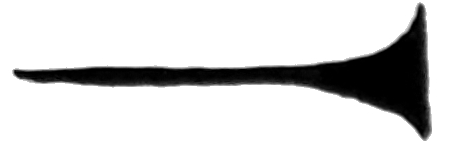
\includegraphics[width=.25\textwidth]{images/10-env1.png} 

    %     \vspace{25pt}
        
    %         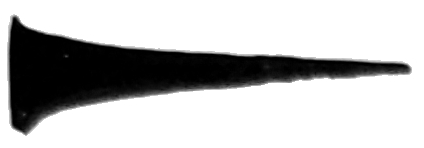
\includegraphics[width=.25\textwidth]{images/10-env2.png} 

    %     \vspace{25pt}
    %         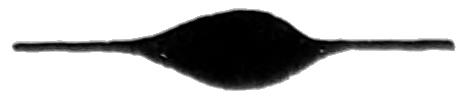
\includegraphics[width=.25\textwidth]{images/10-env3.png} 

    %     \vspace{25pt}
    %         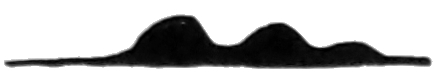
\includegraphics[width=.25\textwidth]{images/10-env4.png} 

    %     \vspace{25pt}
    %         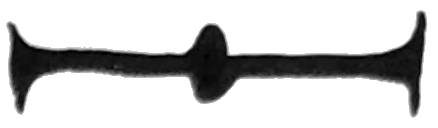
\includegraphics[width=.25\textwidth]{images/10-env5.png} 

    %     \vspace{25pt}
    %         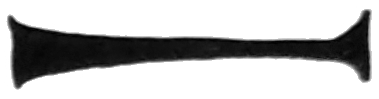
\includegraphics[width=.25\textwidth]{images/10-env6.png}

    %     \vspace{25pt}
    %         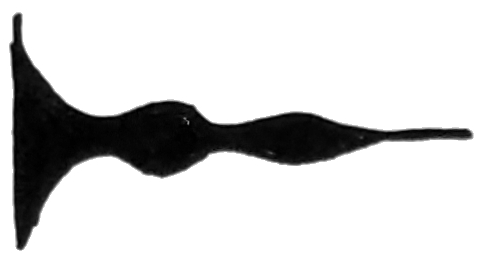
\includegraphics[width=.25\textwidth]{images/10-env10.png}

    %     \vspace{25pt}
    %         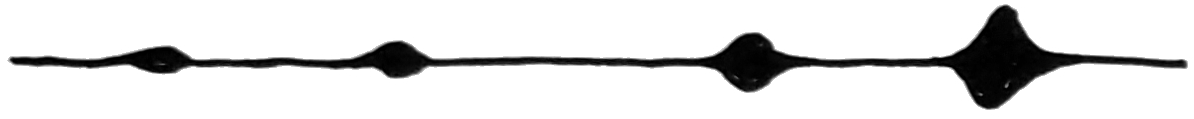
\includegraphics[width=.4\textwidth]{images/10-env7.png} 

    %     \vspace{25pt}
    %         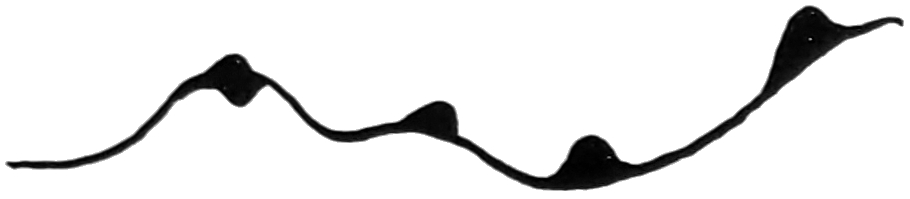
\includegraphics[width=.4\textwidth]{images/10-env8.png} 

    %     \vspace{25pt}
    %         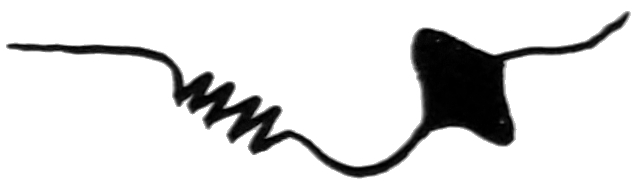
\includegraphics[width=.4\textwidth]{images/10-env9.png} 
            
    % \end{multicols}
    
\newpage


        \section[Timbral flux]{Timbral flux\\\small\textit{visual texture :: sonic texture}}

        %\vspace{15pt}

            \begin{center}
            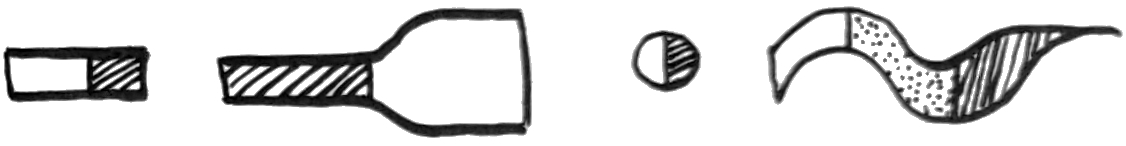
\includegraphics[width=.8\textwidth]{images/02-timbre1.png}\circledfootnote{{from left to right: change timbre on a single pitch at a fixed dynamic; change timbre on a single pitch while getting louder; change timbre in the middle of a short attack; change timbre twice over the course of this legato phrase}}
            \end{center}

            \begin{center}
            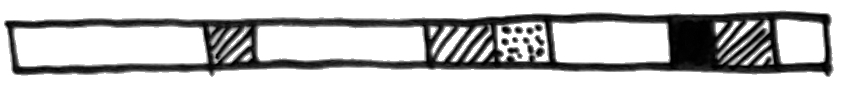
\includegraphics[width=.6\textwidth]{images/02-timbre2.png}\circledfootnote{{change timbre multiple times throughout this long-tone}}
            \end{center}

            

            A change in the \textbf{``visual'' \gls{texture}} of a \gls{dot}, \gls{line}, or \gls{curve} is used to indicate a change in \textbf{timbre} (the precise details of which are left up to the performer). This might mean over-pressure (for strings), muting (for brass) or any other means of modulating \gls{timbre} the player deems fit. 

            Markings indicating a change in timbre need not be consistent across a performance---only, ideally, across a given gesture. For instance, in the diagram above, a player may begin the initial gesture with a clean, dark timbre where the glyph becomes hatched. At the onset of the subsequent gesture, however, the hatched texture of this new glyph could be interpreted as a new timbre entirely.

\newpage

    \section[Simultaneity lines]{Simultaneity lines\\\small\textit{tying events together}}
    

            
        In scored music which is often unmetered, \textbf{gestural simultaneity} becomes an important notational concern. When two events are meant to coincide, a dashed vertical \gls{line} connects those two events (be they the beginnings or endings or middles of gestures). These most often occur \textbf{between} two players, but will also occur in a single player's music to clarify an otherwise ambiguous passage. 

            \begin{center}
            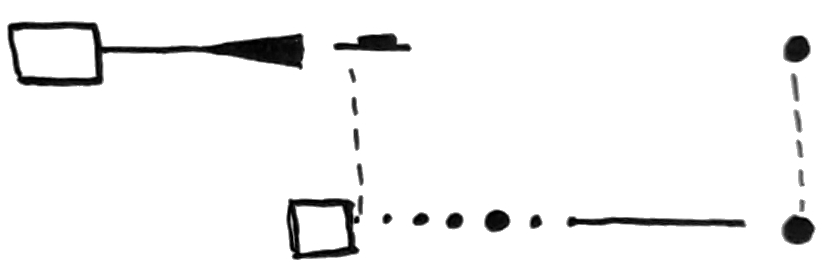
\includegraphics[width=.7\textwidth]{images/02-sim2.png}
            \end{center}

        \noindent In the figure above, simultaneity lines are shown between the two players. The first player begin with a crescendo on a single tone with an abrupt cutoff; the second player begins \textbf{as soon as} the first player rests. After a short passage, both play a staccato attack together.
        
            %\vspace{15pt}

            \begin{center}
            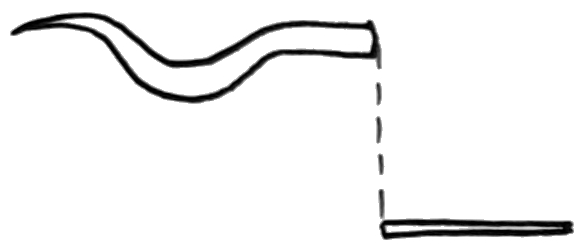
\includegraphics[width=.4\textwidth]{images/02-sim.png}\circledfootnote{{play this contour then (without a pause) jump down to a steady low pitch}}
            \end{center}
        
       \noindent Without the dashed line in the figure above, it would be difficult to see at a glance if appreciable space exists between the low tone and the high one---thus a line is used to show that the high tone should follow immediately rather than after a short rest.

    \subsection*{Cuing}
    
        Occasionally, for ease of rehearsal and performance,\textbf{ markers in the form of stars} will be placed above synchronous events to indicate potential \textbf{\gls{cue} points}---for instance, simultaneous attacks following fermata'd rests.


            \begin{center}
                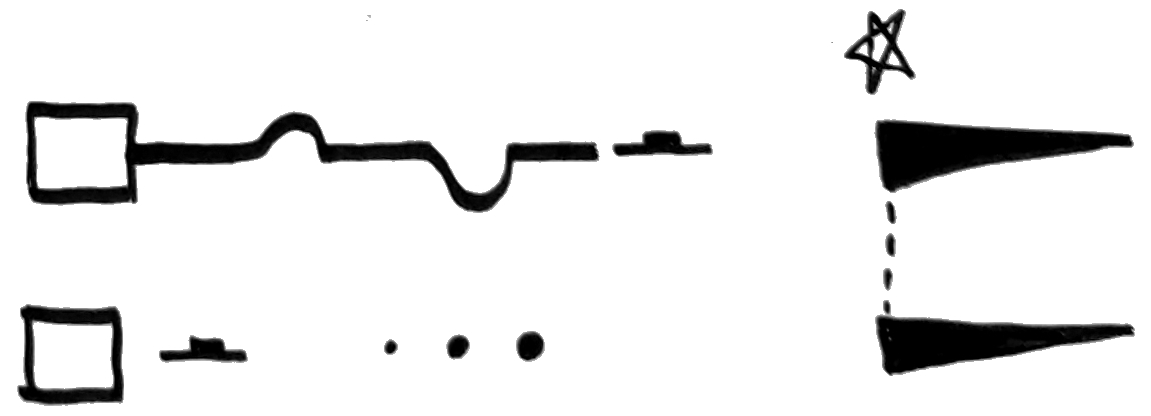
\includegraphics[width=.7\textwidth]{images/08-star.png}\circledfootnote{Player 1 begins while Player 2 rests. Player 2 plays three short attacks at an unspecified position. Then, following a rest, both players re-enter simultaneously at the star.}
            \end{center}

    \newpage
        
    \section[Lollipops]{Lollipops\\\small\textit{representing changing parameters}}

            %\vspace{15pt}
            
            \begin{center}
            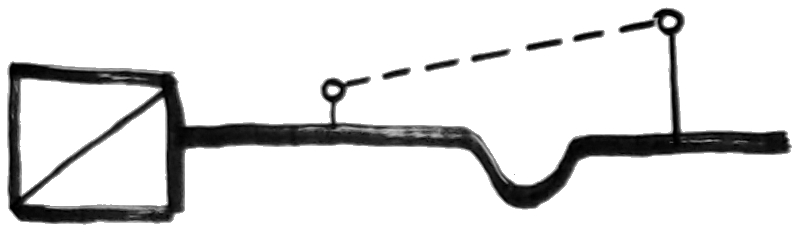
\includegraphics[width=.5\textwidth]{images/02-lolly1.png}\circledfootnote{{an undefined parameter increases while this simple pitch contour is performed}}
            \hspace{15pt}
            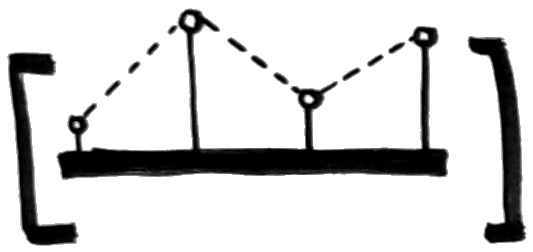
\includegraphics[width=.5\textwidth]{images/02-lolly2.png}\circledfootnote{{an undefined parameter oscillates on a single pitch in an in-this-manner bracket}}
            \end{center}


        ``\textbf{Lollipop}'' glyphs are used to indicate some \textbf{modifier}, i.e. a parameter which varies over the course of a gesture. As mentioned in Section 2.3 (\textbf{The box}), this parameter will usually be indicated in the southeast corner of the ``\gls{box}'' clef and may include things like bow position, airiness, noisiness, amount of mute, etc. Any parameter which could conceivably be represented with a single increasing and decreasing value could happily be encoded with \gls{lollipop}s:

        %\vspace{15pt}

        \begin{center}
            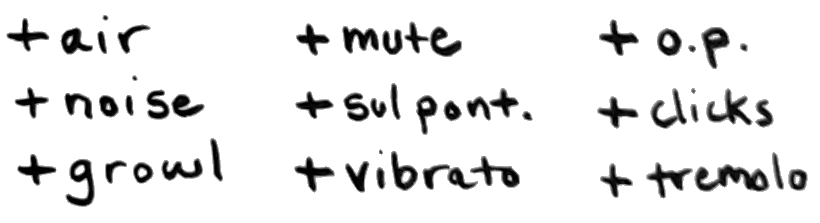
\includegraphics[width=.8\textwidth]{images/02-lolly4.png} 
        \end{center}
        
        The first lollipop will appear where the changing parameter should begin and a dotted line will indicate the \textbf{relative degree} of that technique. I typically use strictly linear progressions from one lollipop to the next rather than curved lines---although there is no hard-and-fast rule saying this must be the case. A dashed line without an accompanying terminator indicates that the parameter should remain at its last value until ``reset'' at the next gesture. In the absence of any further information in subsequent gestures, one should assume that the lollipop no longer holds.

            %\vspace{15pt}
            \begin{center}
            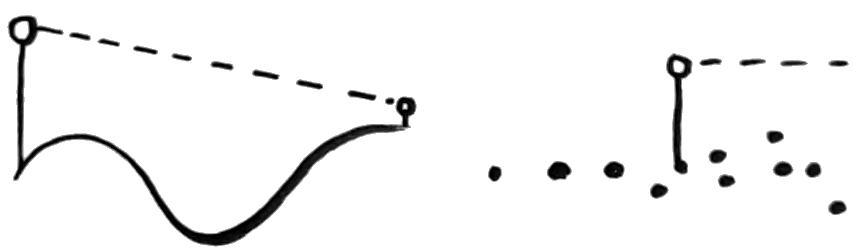
\includegraphics[width=.8\textwidth]{images/02-lolly3.png}\circledfootnote{{a parameter decreases over the course of a legato phrase; the same parameter is specified again in the middle of a staccato passage and remains constant}}
            \end{center}
            
        As shown in the graphic below, two simultaneous changing parameters are relatively easy to deploy as long as both are clearly labelled. I suspect that attempting to represent more than two parameters would render a passage unwieldy and would perhaps best be saved for a different sort of compositional practice.

            %\vspace{15pt}
            \begin{center}
            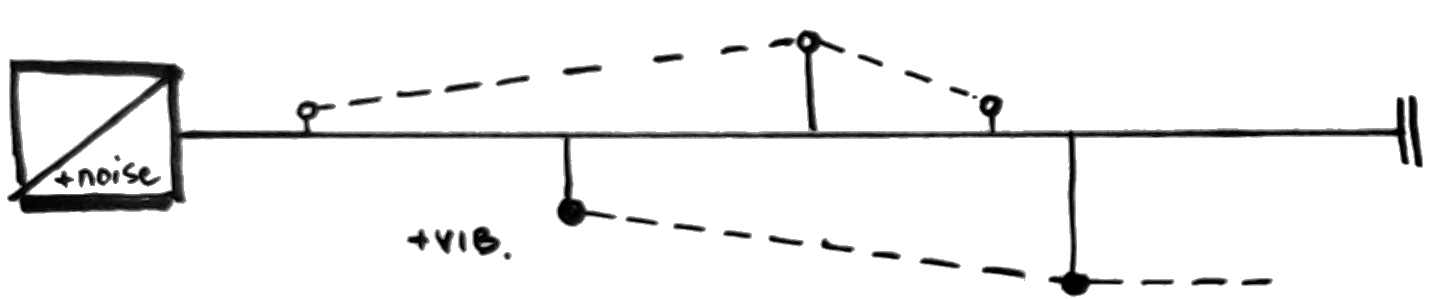
\includegraphics[width=.9\textwidth]{images/02-lolly5.png}\circledfootnote{{a single pitch has two parameters modified: noisiness is represented by the top lollipop since it's given in the box; vibrato is represented by the bottom lollypop and is defined by the tag to the left}}
            \end{center}

    \newpage

    \section[Relational signs]{Relational signs\\\small\textit{situationally dynamic improvisation}}

        A specific class of glyphs, \textbf{\gls{relational signs}} indicate some relationship between the currently active material and some other material---either another player's or one's own. In the following list, I have attempted to encompass quite a wide range of relational possibilities without developing so many new symbols that they begin to tax the performer's recall abilities. For ease of execution, I recommend re-articulating the meanings of these glyphs in individual scores.

    \begin{center}
    \textbf{some common examples}
    
    \vspace{10pt}
    \footnotesize
    \begin{tblr}{
        width=\textwidth,
        cells={valign=m, halign=l},
        colspec={X[3] | X[3] | X[6]},
        column{1}={halign=r},
        column{2}={halign=c}
        }
        $\vcenter{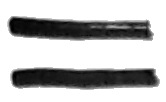
\includegraphics[width=.1\textwidth]{images/03-match.png}}$ & \textit{match x} & match target's playing (in terms of pitch, rhythm, timbre, etc.) \\
        $\vcenter{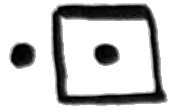
\includegraphics[width=.1\textwidth]{images/03-ignore.png}}$ & \textit{ignore x} & perform as though target is not present \\
        $\vcenter{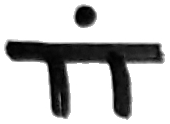
\includegraphics[width=.1\textwidth]{images/03-support.png}}$ & \textit{support x} & perform in such a way that target serves as the ``foreground'' to your ``background'' \\
        $\vcenter{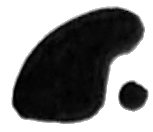
\includegraphics[width=.1\textwidth]{images/03-dominate2.png}}$ & \textit{dominate x} & perform in such a way that target becomes ``background'' to your ``foreground'' \\
        $\vcenter{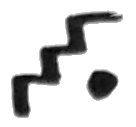
\includegraphics[width=.1\textwidth]{images/03-build.png}}$ & \textit{build upon x} & develop an idea presented by target (either another player or a previous gesture) \\
        $\vcenter{
\includegraphics[width=.2\textwidth]{images/03-echo.png}}$ & \textit{echo x} & serve as an ``echo'' to target player or gesture \\
        $\vcenter{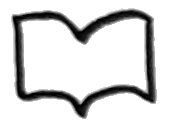
\includegraphics[width=.1\textwidth]{images/03-memorize.png}}$ & \textit{memorize x} & commit (some aspect(s) of) target to memory for later use \\
        $\vcenter{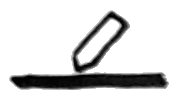
\includegraphics[width=.1\textwidth]{images/03-recall.png}}$ & \textit{recall x} & recall that which was committed to memory in the ``memorize'' gesture
    \end{tblr}
    \end{center}
    
    % \begin{tabular}{l|l}
    %     $\vcenter{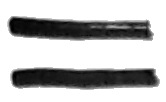
\includegraphics[width=.1\textwidth]{images/03-match.png}}$ & \textit{match x} \\
    %     $\vcenter{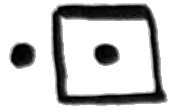
\includegraphics[width=.1\textwidth]{images/03-ignore.png}}$ & \textit{ignore x} \\
    %     $\vcenter{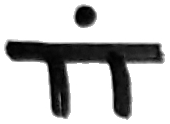
\includegraphics[width=.1\textwidth]{images/03-support.png}}$ & \textit{support x} \\
    %     $\vcenter{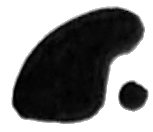
\includegraphics[width=.1\textwidth]{images/03-dominate2.png}}$ & \textit{dominate x} \\
    %     $\vcenter{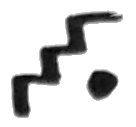
\includegraphics[width=.1\textwidth]{images/03-build.png}}$ & \textit{build upon x} \\
    %     $\vcenter{
\includegraphics[width=.2\textwidth]{images/03-echo.png}}$ & \textit{echo x} \\
    %     $\vcenter{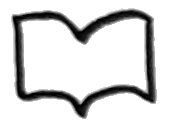
\includegraphics[width=.1\textwidth]{images/03-memorize.png}}$ & \textit{memorize x} \\
    %     $\vcenter{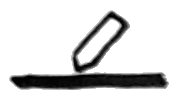
\includegraphics[width=.1\textwidth]{images/03-recall.png}}$ & \textit{recall x}
    % \end{tabular}

    % \begin{description}
    % \item[Most commonly-used examples:]
    % \end{description}
    %     \begin{itemize}
    %     \small
    %         \item \textit{Match $x$} \hspace{10pt} $\vcenter{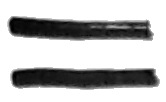
\includegraphics[width=.1\textwidth]{images/03-match.png}}$ \\ match target's playing (in terms of pitch, rhythm, timbre, etc.)
    %         \item \textbf{Ignore ``x''} \hspace{10pt} $\vcenter{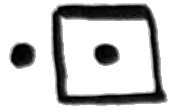
\includegraphics[width=.1\textwidth]{images/03-ignore.png}}$ \\ perform as though target is not present
    %         \item \textbf{Support ``x''} \hspace{10pt} $\vcenter{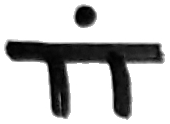
\includegraphics[width=.1\textwidth]{images/03-support.png}}$ \\ perform in such a way that target serves as the ``foreground'' to your ``background''
    %         \item \textbf{Dominate ``x''} \hspace{10pt} $\vcenter{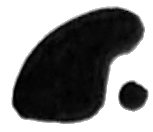
\includegraphics[width=.1\textwidth]{images/03-dominate2.png}}$ \\ perform in such a way that target becomes ``background'' to your ``foreground''
    %         \item \textbf{Build upon ``x''} \hspace{10pt} $\vcenter{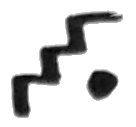
\includegraphics[width=.1\textwidth]{images/03-build.png}}$ \\ develop an idea presented by target (either another player or a previous gesture)
    %         \item \textbf{Echo ``x''} \hspace{10pt} $\vcenter{
\includegraphics[width=.2\textwidth]{images/03-echo.png}}$ \\ serve as an ``echo'' to target player or gesture
    %         \item \textbf{Memorize ``x''} \hspace{10pt} $\vcenter{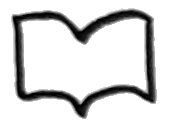
\includegraphics[width=.1\textwidth]{images/03-memorize.png}}$ \\ commit (some aspect(s) of) target to memory for later use
    %         \item \textbf{Recall ``x''} \hspace{10pt} $\vcenter{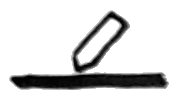
\includegraphics[width=.1\textwidth]{images/03-recall.png}}$ \\ recall that which was committed to memory in the ``memorize'' gesture
    %     \end{itemize}

    %\vspace{15pt}

\noindent ...and here are some potentially powerful but as-yet-unused examples:

\begingroup
    \begin{center}
        \textbf{unused (but interesting) examples}
        
        \vspace{10pt}
        \footnotesize
        \begin{tblr}{
            width=\textwidth,
            cells={valign=m, halign=l},
            colspec={X[4] | X[4] | X[6]},
            column{1}={halign=l},
            column{2}={halign=l}
            }
            $\vcenter{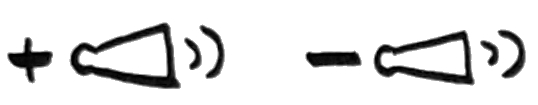
\includegraphics[width=.25\textwidth]{images/03-louder.png}}$ & \textit{louder/softer} & \\
            $\vcenter{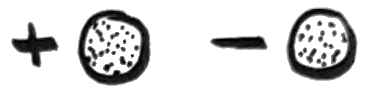
\includegraphics[width=.25\textwidth]{images/03-denser.png}}$ & \textit{denser/rarer} & \\
            $\vcenter{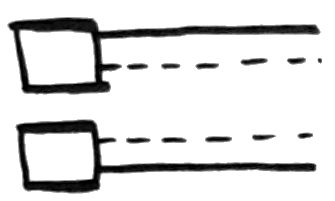
\includegraphics[width=.2\textwidth]{images/03-higher.png}}$ & \textit{higher/lower} & \\
            $\vcenter{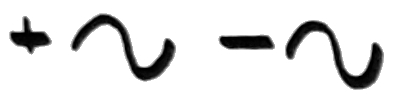
\includegraphics[width=.2\textwidth]{images/03-purer.png}}$ & \textit{purer/noisier} & \\
            $\vcenter{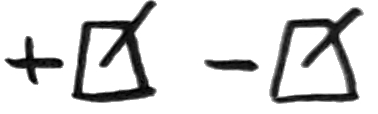
\includegraphics[width=.2\textwidth]{images/03-faster.png}}$ & \textit{faster/slower} & \\
            $\vcenter{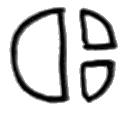
\includegraphics[width=.1\textwidth]{images/03-decompose.png}}$ & \textit{decompose x} & perform \textit{x} but with ``pieces missing'' or in some way incomplete or broken-down \\
            $\vcenter{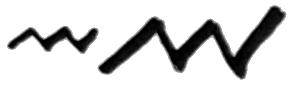
\includegraphics[width=.2\textwidth]{images/03-exaggerate.png}}$ & \textit{exaggerate x} & perform \textit{x} but in some way exaggerated (wider contours, louder, etc.) \\
            $\vcenter{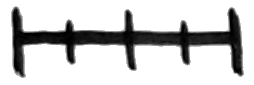
\includegraphics[width=.2\textwidth]{images/03-rhythmicize.png}}$ & \textit{rhythmicize x} & perform \textit{x} but now conforming to some sort of rhythmic grid \\
            $\vcenter{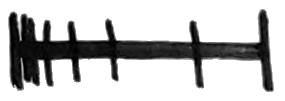
\includegraphics[width=.2\textwidth]{images/03-rubato.png}}$ & \textit{rubato x} & perform \textit{x} but now without regard to a rhythmic grid \\
            $\vcenter{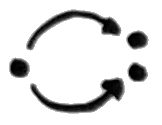
\includegraphics[width=.15\textwidth]{images/03-multiply.png}}$ & \textit{multiply x} & take a fragmentary gesture \textit{x} and multiply it indefinitely \\
            $\vcenter{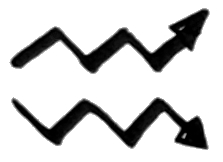
\includegraphics[width=.15\textwidth]{images/03-counterpoint.png}}$ & \textit{counterpoint x} & provide counterpoint (rhythmically, pitch-wise, timbrally) to \textit{x}
        \end{tblr}
        \end{center}
\endgroup


    \newpage
    
    In context, the relational sign will be placed at the bottom-left of an accompanying gesture and will use an \gls{arrow} to indicate its point of reference, be it another player's gesture or one's own.
    
            \begin{center}
            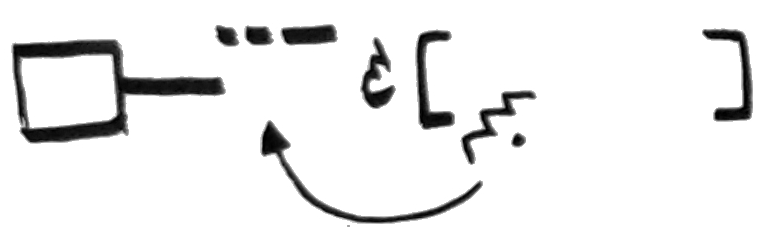
\includegraphics[width=.4\textwidth]{images/05-relation1.png}\circledfootnote{{build upon previous gesture}}
            \end{center}

            \vspace{15pt}

            \begin{center}
            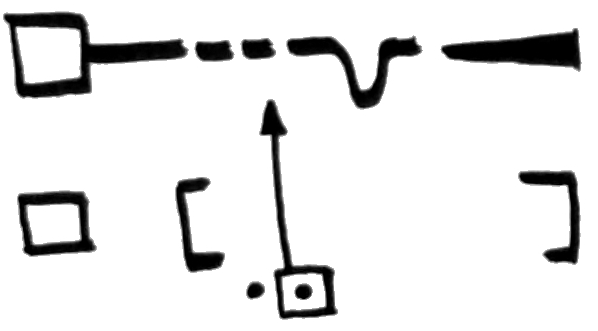
\includegraphics[width=.4\textwidth]{images/05-relation2.png}\circledfootnote{{ignore other player's gesture}}
            \end{center}

            \vspace{15pt}
            
            \begin{center}
            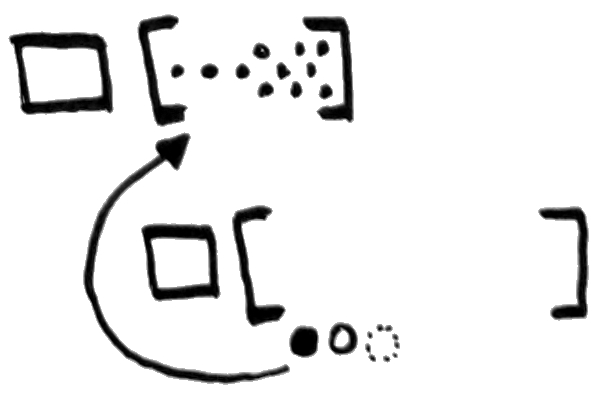
\includegraphics[width=.4\textwidth]{images/05-relation3.png}\circledfootnote{{echo other player's gesture}}
            \end{center}

\newpage

    \section{Other global signs}

        \subsection[Incorporating pitched material]{Incorporating pitched material\\\small\textit{notational hybridity}}

        %\vspace{15pt}

            \begin{center}
            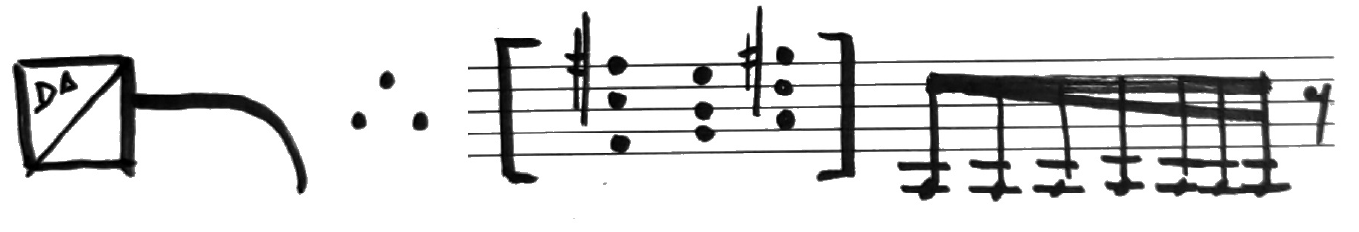
\includegraphics[width=.9\textwidth]{images/06-Artboard 3.png}\circledfootnote{{over a D major chord play a falling gesture followed by three staccato attacks, then play something like the given chords, then play this accelerando gesture on A3}}
            \end{center}        

            A central goal of this system is a more-or-less seamless integration of traditionally notated materials with new open glyphs.
            
           \textbf{\Gls{Pitched material}} may be incorporated in several ways. Rarely, notation may be included which is fully rendered with meter, tempo, dynamics, etc. However, more commonly, several of these factors are omitted in favor of fixed pitches to be played in a given order but with no rhythmic/durational information. Other times, no order is specified.
           
                \begin{center}
                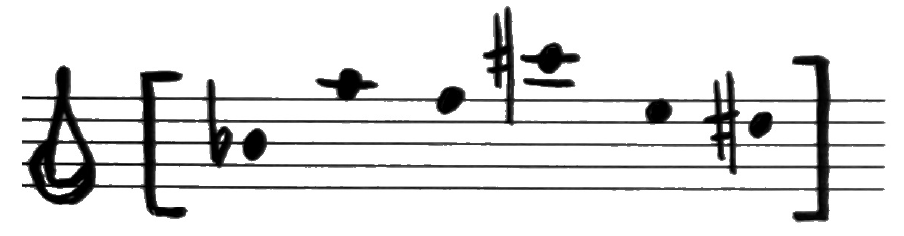
\includegraphics[width=.75\textwidth]{./images/non_specific_pitches.png}\circledfootnote{{play something using these pitches with no particular rhythm}}
                \end{center}
            
           In instances where rhythms are given, these rhythms are to be performed proportionally unless otherwise noted.

            \begin{center}
            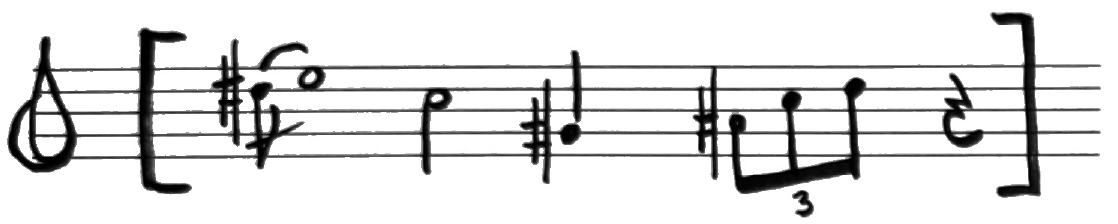
\includegraphics[width=.9\textwidth]{images/06-Artboard 2.png}\circledfootnote{{play something like these pitches/rhythms proportionally (not necessarily in sync with anyone else)}}
            \end{center}



\newpage
            
        \subsection{``Relative'' rests}

            %\vspace{15pt}
            \begin{center}
            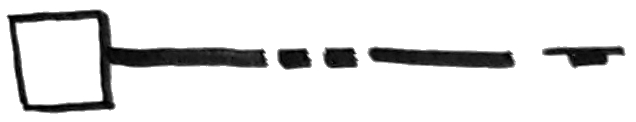
\includegraphics[width=.6\textwidth]{images/03-rest.png}\circledfootnote{{one interrupted pitch followed by a long rest}}
            \end{center}        

            Often, players will see eighth-, quarter-, half-, and whole-rests ``floating'' amidst other open glyphs. Unless otherwise marked, these \textbf{floating rests} are to be understood as ``psychological'' proportional indicators rather than as concrete durational values---i.e. eighth = quite short rest, quarter = longer rest, whole = quite long rest, etc.
            
            %\vspace{15pt}
            \begin{center}
            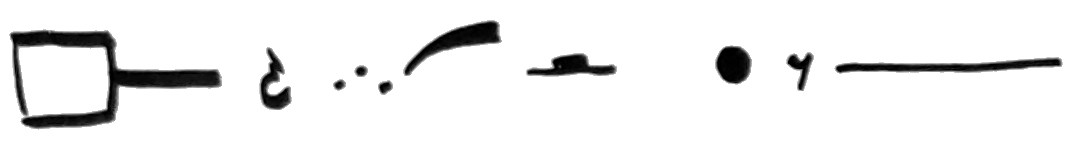
\includegraphics[width=.9\textwidth]{images/03-rest2.png}\circledfootnote{{play this gesture with rests of various proportional lengths}}
            \end{center}        

\newpage
            
        \subsection{Repeats}

            When a repeat is used to enclose a gesture, the player ought to loop that gesture (to the best of their ability) rather than extend and develop it. The duration of the repeated gesture will be (as usual) denoted by the amount of territory enclosed by the repeats, while the duration of the overall repetition will be indicated with a simple \gls{arrow} or a strict \textbf{number of repeats (2x, 3x, etc.)}.

            %\vspace{15pt}
            \begin{center}
            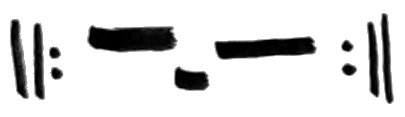
\includegraphics[width=.5\textwidth]{images/03-repeat1.png}\circledfootnote{{repeat this long-short-long figure}}
            \end{center}

            %\vspace{15pt}
            \begin{center}
            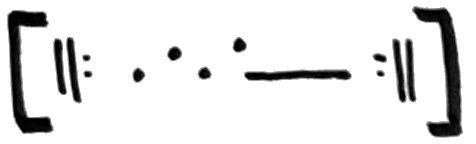
\includegraphics[width=.5\textwidth]{images/03-repeat2.png}\circledfootnote{{``in the manner of'' a repetition of this staccato-then-single-tone phrase}}
            \end{center}

\newpage
            
        \subsection[Transition arrow]{Transition arrow\\\small\textit{gradual becoming}}

            This thick, more elaborate \gls{arrow} is used to indicate that a player should \textbf{transition gradually} (rather than jump-cut) from one ``sound world'' into another using whatever means they deem appropriate. The length of the arrow indicates the proportional duration of the transition period.

            %\vspace{15pt}
            \begin{center}
            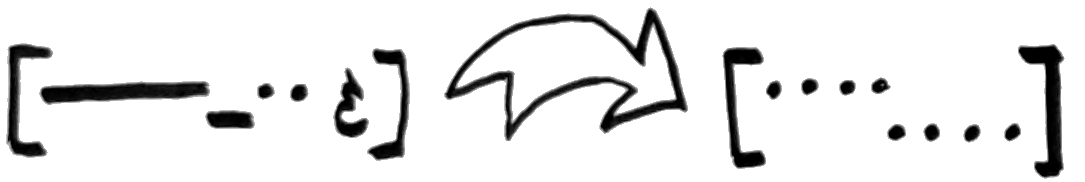
\includegraphics[width=.9\textwidth]{images/03-transition.png}\circledfootnote{{transition rather quickly from a mix of longer and shorter attacks to consistent short attacks in a narrow pitch band}}
            \end{center}  

\newpage
            
        \subsection[``Grid'' indications]{``Grid'' indications\\\small\textit{rhythmic/arrhythmic}}

            These symbols are used to indicate that improvisation should occur either \textbf{metronomically} (``on a grid''---i.e. using an imagined isochronous pulse governing performed rhythms),
            
            %\vspace{15pt}
            \begin{center}
            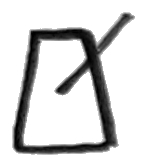
\includegraphics[width=.1\textwidth]{images/08-met1.png}
            \end{center}  

\noindent \textbf{semi-metronomically} (semi-pulsed),

            %\vspace{15pt}
            \begin{center}
            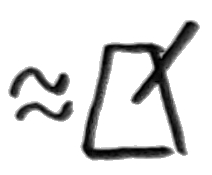
\includegraphics[width=.15\textwidth]{images/08-met2.png}
            \end{center}  


\noindent or \textbf{unmetered}. 

            %\vspace{15pt}
            \begin{center}
            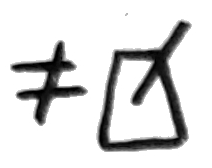
\includegraphics[width=.15\textwidth]{images/08-met3.png}
            \end{center}  
            
As a general rule, gestures are to be understood as unmetered unless otherwise noted. Furthermore, two players simultaneously playing \textbf{metronomic} gestures \textit{need not} match tempos unless the ``match ``x'''' glyph is also present. Rather, they should each strive to maintain a consistent, independent tempo until unmetered play resumes.

            %\vspace{15pt}
            \begin{center}
            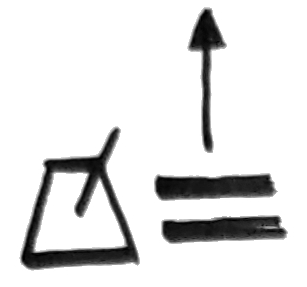
\includegraphics[width=.2\textwidth]{images/08-met4.png}\footnote{As usual, an arrow will be used to indicate the point of reference for the \textbf{match x} relational sign.}
            \end{center}  

\newpage
            
        \subsection{``Interruptions''}

            Two symbols are used to indicate \textbf{interruptions} of the ongoing flow of a gesture.

            \begin{center}
            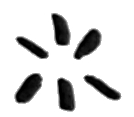
\includegraphics[width=.1\textwidth]{images/05-interruption3.png} 
            \end{center}
            
            \noindent indicates an \gls{interruption} ``\textbf{in time}'' which interjects sound of the player's choosing in such a way that the proportionality of the gesture group is unaltered---often a sudden burst unrelated to the rest of the music in question.
            
            On the other hand, 
            
            \begin{center}
            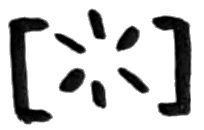
\includegraphics[width=.15\textwidth]{images/05-interruption4.png}
            \end{center}
            
            \noindent indicates an interruption ``\textbf{out of time}''---i.e. of open duration, breaking not only the sonic flow, but also the \textit{temporal} flow of the gesture.

\setcounter{footnote}{0}
\chapter{Family-specific glyphs}
\label{ch:family-specific}
\newpage

    \section{Polyphonic Instruments}

        \subsection{Chords and chord-density}

        Homophonic gestures (that is, gestures which are primarily composed of vertically-stacked harmonies rather than monophonic single-note lines) present a unique challenge to notation in this scheme, given the scheme's reliance on essentially one-dimensional simple linear figures. As such, generically homophonic material is shown using \textbf{striated dots and contours} which are \gls{texture}d with \textbf{parallel, left-to-right oriented bands}.
        
            \begin{center}
            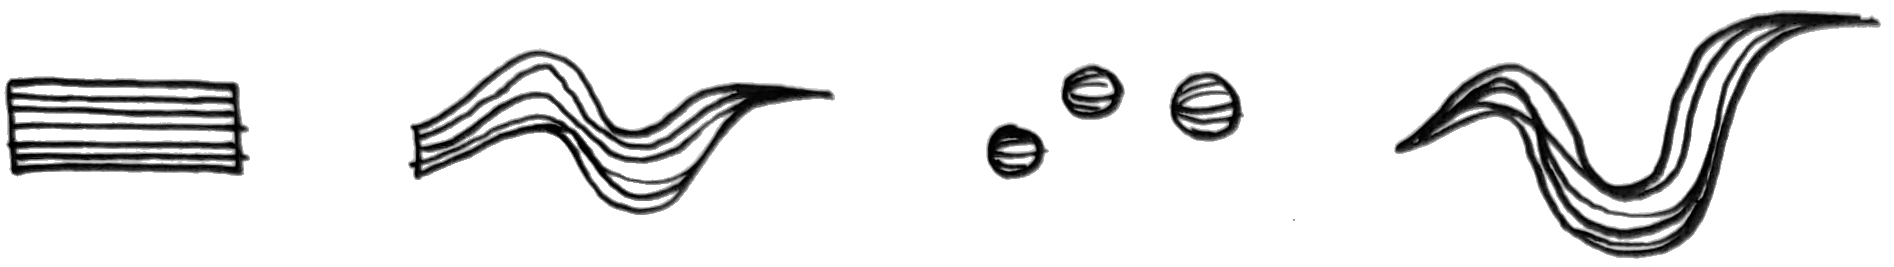
\includegraphics[width=.9\textwidth]{images/04-chords.png}\circledfootnote{{from left to right: long, chordal attack, quite loud; legato figure composed of chords; three short chordal attacks; wider-range chordal legato figure}}
            \end{center}  
            
    As usual, the approximate range of the gesture is given by its position on the y-axis. Note that the striations themselves do not give any particular information as to the intervallic content or chord voicing---these properties, if constrained at all, will be given elsewhere; usually in the accompanying \gls{box} or attached to the gesture with a flag. To this end, a widely-spaced staffless half-note \gls{chord} indicates that the player should favor more open voicings. Converseley, a clustered half-note chord points to tighter, closed voicings.

            \begin{center}
            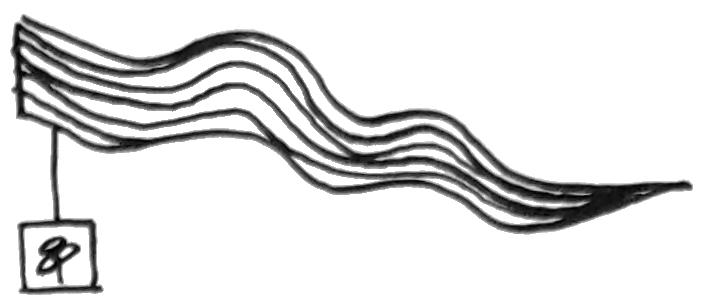
\includegraphics[width=.4\textwidth]{images/04-chords2.png}\circledfootnote{{descending chordal legato passage primarily using ``closed'' or ``cluster'' voicings}}
            \hspace {15pt}
            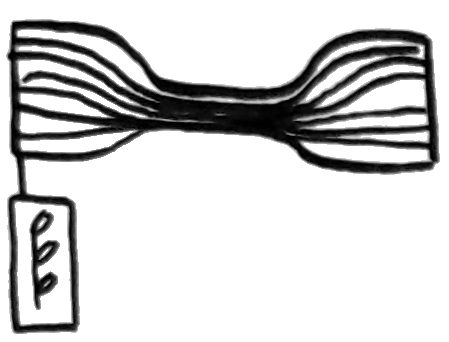
\includegraphics[width=.4\textwidth]{images/04-chords3.png}\circledfootnote{{loud-soft-loud gesture using ``open'' (widely spaced) voicings}}
            \end{center}  

\newpage
        
        
    
    \section{Strings}
    
        \subsection{Harmonics}

            \begin{center}
            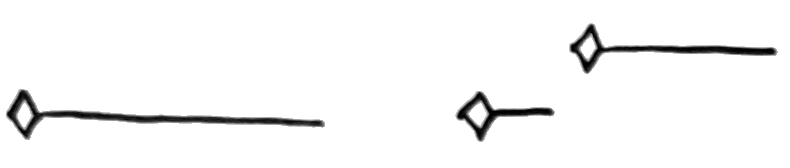
\includegraphics[width=.8\textwidth]{images/04-harmonics.png}\circledfootnote{{plain, unbroken harmonics}} 
            \hspace {15pt}
            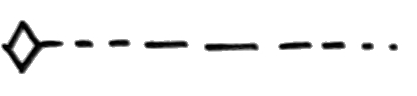
\includegraphics[scale=0.3]{images/04-harmonics2.png}\circledfootnote{{a ``morse-code'' ---i.e. mixed long and short attacks---harmonic}}
            \end{center} 

            Harmonics are indicated by a \textbf{diamond} glyph preceding a duration line. As \gls{harmonic}s tend to be considerably higher than stopped pitches, the harmonic figure in essence temporarily overrides the prescribed range and should be understood to be high- or low-pitch in relation to other harmonics present.

\newpage
            
        \subsection{Double-stops et al.}

            \begin{center}
            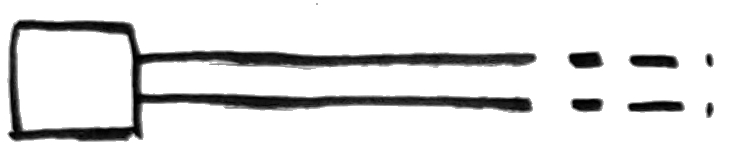
\includegraphics[width=0.7\textwidth]{images/04-doublestops.png}\circledfootnote{{a double stop on a single pitch which is interrupted toward the end of the gesture}} 
            \hspace {15pt}
            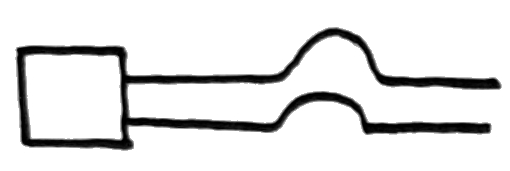
\includegraphics[width=0.5\textwidth]{images/04-doublestops2.png}\circledfootnote{{a double stop which begins and returns to a single pitch}}
            \end{center}

            Double/triple/etc. stops are, predictably, indicated by \textbf{multiple concurrent duration lines}. They may move in parallel or in contrary motion and may feature distinct attack envelopes, etc.

            \begin{center}
            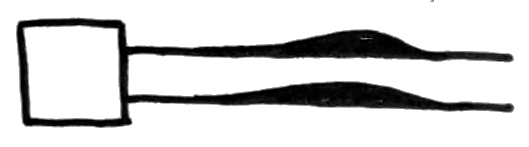
\includegraphics[width=0.5\textwidth]{images/04-doublestops3.png}\circledfootnote{{a double stop which peaks in intensity toward the middle of the gesture}}
            \hspace {15pt}
            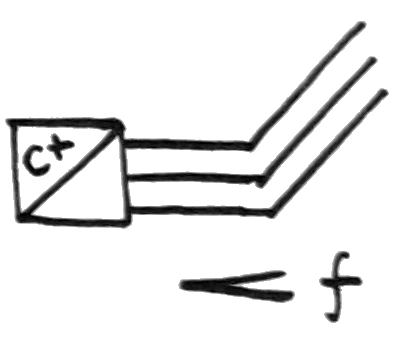
\includegraphics[width=0.4\textwidth]{images/04-doublestops4.png}\circledfootnote{{a triple stop using a C-augmented pitch set which rapidly ascends and gets louder}}
            \end{center}

\newpage

    \section{Winds}

        \subsection{Multiphonics}

            Multiphonics are indicated by a unique glyph (borrowed from Braxton's ``Language Music'' scheme) preceding the duration line. In the absence of other direction, \gls{multiphonic}s should be chosen based on the figure's position on the y-axis. 

            \begin{center}
            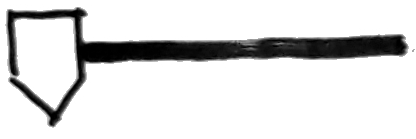
\includegraphics[width=0.4\textwidth]{images/04-multiphonics2.png} \hspace {15pt} 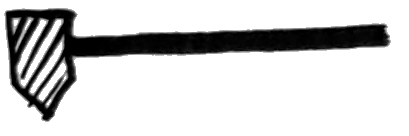
\includegraphics[width=0.4\textwidth]{images/04-multiphonics3.png}\circledfootnote{{two discrete multiphonics in approximately the same register and with the same dynamic}}
            \end{center}

            \noindent In some instances, unspecified but \textbf{discrete} multiphonics are desired. In this case, the initial glyph will be \gls{texture}d using ``timbral change'' glyph textures. These distinctions are local to the gesture, similar to changes in \textbf{timbre (section 2.7)}---i.e. the multiphonic signified by the hatched symbol need not be consistent across the entire piece; only until the \textbf{box} clef indicates the start of a new gesture.

            %\vspace{15pt}
            \begin{center}
            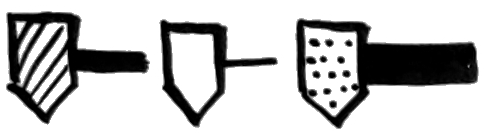
\includegraphics[width=.5\textwidth]{images/04-multiphonics4.png}\circledfootnote{{three discrete multiphonics at different dynamics}}
            \end{center}
            
\newpage

    \section{Brass}

        \subsection{Mutes}

            \begin{center}
            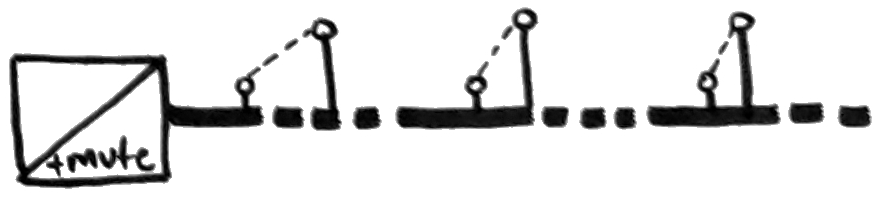
\includegraphics[width=.9\textwidth]{images/mutelolly.png}\circledfootnote{{interrupted attack(s) on a single pitch while opening/closing the mute}}
            \end{center}

            The use of mutes is certainly permitted/encouraged in the absence of other instructions. Sometimes, though, the use of a plunger-style (\textbf{dynamic}) mute is called for expressly in the score in the \textbf{southeast} corner of \textbf{the \gls{box}} (``+mute''), in which case a \textbf{\gls{lollipop}} will indicate the extent/velocity of mute movement.

            Other (\textbf{static}) mutes will be indicated using text as usual.
\newpage

    \section{Percussion}
        \subsection*{Special considerations for percussion}

            There are special challenges inherent in notating improvised percussion music. The percussionist has myriad instruments at their disposal with a concomitant wide array of techniques which often necessitate case-by-case notation schemes (see research by Lindsay Vickery et al.\footnote{Vickery, Lindsay et al., ``Expanded Percussion Notation in Recent Works by Cat Hope, Stuart James and Lindsay Vickery,'' 2017}) As such, I take a generalist, instrument-agnostic approach by mapping percussion instruments to the y-axis according to their average spectral content. If a particular instrument is desired for a given gesture, then an \gls{arrow} should be used to connect that gesture to the appropriate name or pictogram of the instrument.
        
        \subsection{Drum kit}

            In the case of the drum kit, for instance, one might include a small diagram as part of the ``clef'' figure which includes explicit mapping-regions illustrated by \textbf{pictographic instruments}.

          %\vspace{15pt}


          In the figure below: typical trap kit components loosely arranged according to spectral content. Top to bottom: crash/splash; ride; snare; tom; bass. These may be changed to suit intended trap kit setup.

            \begin{center}
            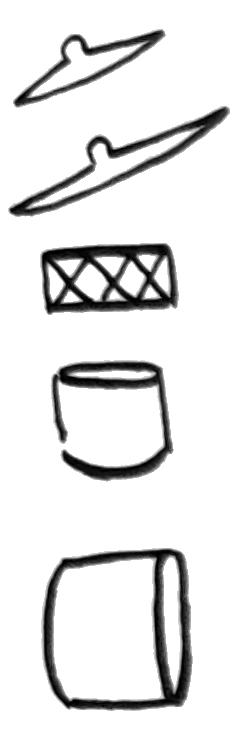
\includegraphics[width=.1\textwidth]{images/05-drums.png}
            \end{center}


\noindent Here shown in context:

            %\vspace{15pt}
            \begin{center}
            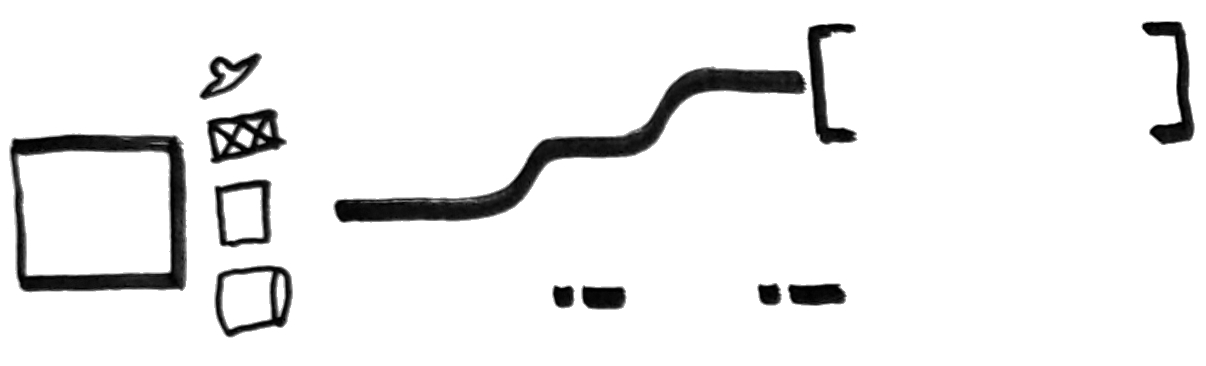
\includegraphics[width=.75\textwidth]{images/05-drums2.png}\footnote{The ``clef'' illustrates approximate regions of play corresponding to height of the line. In this case, the gesture may be interpreted as \textit{ascending in spectral space while playing low attacks (probably on the kick drum); then, open improvisation in the upper register}}
            \end{center}


    \subsection{Other percussion}

        Custom \gls{pictograms} may serve a valuable role in efficiently communicating a desired technique. Shown below are just a few that have been deployed in past pieces.

            \begin{center}
            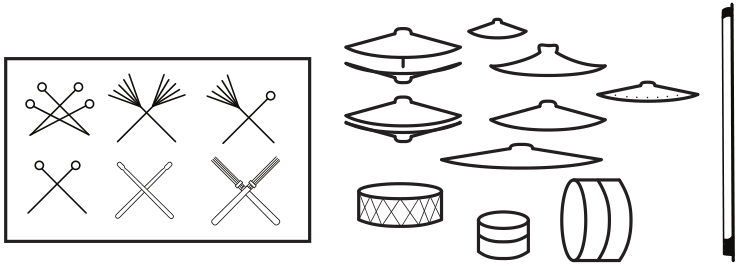
\includegraphics[width=.9\textwidth]{images/percussionpictograms.png}\footnote{Left in box: various sticks/mallets\\Center: various cymbals/drums\\Right: bow}
            \end{center}



            
\newpage

\chapter{Room for development}
\label{ch:development}

    \subsection{The voice}

    Though there is nothing stopping an intrepid vocalist from performing open-instrumentation pieces featuring this style of notation, the scheme has yet to expand into vocal music proper. Of particular interest might be glyphs which pictographically represent common ``vowel shapes'' or vocal formants, as well as some elegant means of providing pools of available syllables/words/phrases which might be attached to particular gestures.
    
    \subsection{Electronic instruments}

    Given their unmatched potential for sonic diversity, electronic instruments pose the thorniest problem for efficient, broadly-applicable notation. Again, there is very little that would prevent an electronics-specialist from performing instrument-agnostic scores. However, to fully take advantage of the vast timbral range encompassed by analog synthesizers, samplers, software instruments, etc., the composer must often develop bespoke solutions to fit individual instruments/instrumentalists.

    One solution might be to more concretely map graphic \gls{texture}s to sonic ones. For example, one might encode the process of increasing grain size (for a granular synthesis patch) with a less-and-less-dense field of dots filling in a pitch curve. Perhaps the presence or absence of white noise in a signal could be signified by shades of gray. These are, of course, kindergarten-level analogies which do not even approach the level of sophistication possible with modern electronic instruments. Nevertheless, work will continue in this arena as opportunities to compose for electronicists present themselves.

    \subsection{Movement}
    Notations for movement and gesture in dance and theater (Labanotation, Benesh Movement Notation, Eshkol-Wachman Movement Notation, etc.) are well-established (if sparsely used), but were not designed to emphasize improvisation or simultaneous music-and-movement performance. Otto-Glyphs lends itself to adaptation for movement-based performance, particularly in cases where performers move and play simultaneously.

%        \subsection{A more robust tablature}

%        [forthcoming]

\clearpage

\setglossarystyle{mystyle}

\printglossary

% \bibliographystyle{IEEEtran}
% \bibliography{references}


\end{document}
